\documentclass[11pt,oneside]{article}

\usepackage[a4paper,margin=27mm,headheight=15pt]{geometry}
\usepackage[T1]{fontenc}
\usepackage[utf8]{inputenc}
\IfFileExists{libertinus.sty}{\usepackage{libertinus}}{\usepackage{lmodern}}
\usepackage{microtype}
\usepackage{amsmath,amssymb,amsthm,mathtools,mathrsfs}
\usepackage{bm}
\usepackage{booktabs,longtable,array,tabularx}
\usepackage{graphicx}
\usepackage{pgfplots}
\usepackage{xcolor}
\usepackage{enumitem}
\usepackage{fancyhdr}
\usepackage{titlesec}
\usepackage{listings}
\usepackage{xurl}
\usepackage{hyperref}
\usepackage[nameinlink,noabbrev]{cleveref}

\definecolor{linkblue}{RGB}{25,75,135}
\definecolor{shadegray}{RGB}{246,247,249}
\definecolor{rulegray}{RGB}{195,201,208}
\pgfplotsset{compat=1.18}
\hypersetup{
  colorlinks=true,
  linkcolor=linkblue,
  citecolor=linkblue,
  urlcolor=linkblue,
  pdftitle={The Decay Envelope of the Rvachev Sinc Product: A Comparative Audit},
  pdfsubject={Audit of four proposed solutions; verified decay spectrum; a corrected constant in the published literature},
  pdfkeywords={Rvachev up-function, Fabius function, sinc product, Fourier decay, Thue-Morse, transfer operator, law of the iterated logarithm}
}

\pagestyle{fancy}
\fancyhf{}
\fancyhead[L]{\small Fourier-decay audit}
\fancyhead[R]{\small\nouppercase{\leftmark}}
\fancyfoot[C]{\thepage}
\renewcommand{\headrulewidth}{0.4pt}

\titleformat{\section}{\Large\bfseries}{\thesection}{0.7em}{}
\titleformat{\subsection}{\large\bfseries}{\thesubsection}{0.7em}{}
\titleformat{\subsubsection}{\normalsize\bfseries}{\thesubsubsection}{0.7em}{}
\setcounter{secnumdepth}{3}
\setcounter{tocdepth}{2}
\setlist[itemize]{leftmargin=2em,itemsep=0.25em,topsep=0.4em}
\setlist[enumerate]{leftmargin=2.3em,itemsep=0.25em,topsep=0.4em}
\setlength{\emergencystretch}{2em}
\allowdisplaybreaks

\newtheorem{theorem}{Theorem}[section]
\newtheorem{proposition}[theorem]{Proposition}
\newtheorem{lemma}[theorem]{Lemma}
\newtheorem{corollary}[theorem]{Corollary}
\newtheorem{conjecture}[theorem]{Conjecture}
\theoremstyle{definition}
\newtheorem{definition}[theorem]{Definition}
\newtheorem{algorithm}[theorem]{Algorithm}
\newtheorem{example}[theorem]{Example}
\theoremstyle{remark}
\newtheorem{remark}[theorem]{Remark}
\newtheorem{warning}[theorem]{Warning}
\newtheorem{finding}[theorem]{Finding}
\crefname{finding}{finding}{findings}
\Crefname{finding}{Finding}{Findings}

\newcommand{\R}{\mathbb R}
\newcommand{\C}{\mathbb C}
\newcommand{\Q}{\mathbb Q}
\newcommand{\N}{\mathbb N}
\newcommand{\Z}{\mathbb Z}
\newcommand{\Up}{\operatorname{up}}
\newcommand{\sinc}{\operatorname{sinc}}
\newcommand{\e}{\mathrm e}
\newcommand{\ii}{\mathrm i}
\newcommand{\dd}{\,\mathrm d}
\newcommand{\Var}{\operatorname{Var}}
\newcommand{\E}{\mathbb E}
\newcommand{\Prob}{\mathbb P}
\newcommand{\bigO}{\mathcal O}
\newcommand{\smallo}{o}
\newcommand{\supp}{\operatorname{supp}}
\newcommand{\sgn}{\operatorname{sgn}}
\newcommand{\vtwo}{v_2}
\newcommand{\repo}{\nolinkurl{Analysis/FabiusFunction}}
\newcommand{\lean}[1]{%
  \ifmmode\text{\nolinkurl{#1}}\else\nolinkurl{#1}\fi}
\newcommand{\T}{T}
\newcommand{\Lop}{\mathcal L}

\newenvironment{boxedremark}{%
  \par\smallskip\noindent\begin{center}\begin{minipage}{0.94\textwidth}%
  \color{black}\hrule\vspace{0.6em}\small
}{%
  \vspace{0.6em}\hrule\end{minipage}\end{center}\smallskip
}

\lstdefinestyle{pseudo}{
  basicstyle=\ttfamily\small,
  backgroundcolor=\color{shadegray},
  frame=single,
  rulecolor=\color{rulegray},
  columns=fullflexible,
  keepspaces=true,
  showstringspaces=false,
  xleftmargin=0.7em,
  xrightmargin=0.7em,
  aboveskip=0.8em,
  belowskip=0.8em
}

\title{\bfseries The Decay Envelope of the Rvachev Sinc Product\\[0.35em]
\large A comparative audit of four proposed solutions, with numerical adjudication\\
and a corrected constant in the published literature}
\author{Comparative analysis for Vladimir Reshetnikov's \texttt{ProveIt} project\\
\small covering the four drafts in \nolinkurl{drafts/rvachev_up_fourier_decay/}}
\date{26 August 2026}

\begin{document}
\maketitle

\begin{abstract}
Mathematics Stack Exchange question 2745497 asks for a positive, analytic,
monotone decreasing gauge $g$ such that the Ces\`aro mean of $|f|/g$ tends to
one, where $f(x)=\prod_{n\ge0}\sinc(\pi x/2^n)$ is the Fourier transform of
Rvachev's up-function.  Four AI-produced documents in this directory propose
solutions.  This audit verifies their overlapping claims numerically and
against the literature, adjudicates their one genuine mutual contradiction,
and states what the answer to the original question actually is.

The four documents agree, correctly, on the universal factor
$\exp(-(\log x)^2/(2\log2))$ and on a spectrum of power corrections
$x^{-\kappa}$ that depends on the meaning of ``amplitude'':
$\kappa_\infty=2.3590148791\ldots$ for the extremal envelope,
$\kappa_2=\log_2(2\pi)=2.6514961295\ldots$ for the quadratic mean,
$\kappa_1=2.7480700149\ldots$ for the arithmetic (Ces\`aro) mean, and
$\kappa_0=3.1514961295\ldots$ for Lebesgue-typical points.  Documents~3
and~4 answer the literal question: the gauge
$g(x)=A_1x^{-\kappa_1}\exp(-(\log x)^2/(2\log2))$ with
$\kappa_1=\tfrac12+\log_2(\pi/\varrho_1)=2.748070014871334\ldots$, where
$\varrho_1=0.661322602060565\ldots$ is the Perron root of an explicit
transfer operator, satisfies the two-sided bounded form of the question and
attains the Ces\`aro limit $1$ along $t=2^k$; but we prove that no gauge
whose within-shell shape stabilizes---in particular no Hardy-field
(``elementary'') gauge---can attain the limit along all $t$: the limit
points trace a nonconstant dyadic-mantissa profile (computed here to span
$[0.9249,1.1133]$), and constancy of the profile would force the
transfer-operator eigenmeasure to be absolutely continuous, contradicting
its singularity, which we prove from the elementary bound
$\varrho_1\ge3^{-1/2}>\tfrac12$.  We add one repair, with proof: with the
same gauge, the \emph{logarithmic} mean
$\frac{1}{\log(t/t_0)}\int_{t_0}^t\frac{|f(x)|}{g(x)}\frac{\dd x}{x}$
converges for all $t\to\infty$, so the multiplicative form of the question
has an exact affirmative answer.

The audit's principal forensic finding concerns the law of the iterated
logarithm.  Document~1 derives, by a martingale argument, per-step variance
$\pi^2/4$ and hence the fluctuation constant $\pi/\sqrt2$; Document~3 quotes
the published Theorem~1.2 of Aistleitner--Hofer--Larcher (Ann.\ Inst.\
Fourier 67 (2017) 637--687), whose constant is $\pi$.  Both cannot be right.
An exact Parseval computation of the paper's own variance functional
(2.9)---confirmed by measurement over exact rational orbits,
$\Var(S_{1000})=2459.5$ against the predictions $2464.1$ for variance
$\pi^2/4$ and $4928.2$ for variance $\pi^2/2$---shows that Document~1 is
correct and that the published equation~(4.5) omits the Parseval factor
$\tfrac12$: the constants in the published Theorems~1.1 and~1.2 should
each be divided by $\sqrt2$.

Two interpretations are developed beyond what any of the four documents
attempts.  The envelope-of-lobe-maxima reading
(\cref{sec:lobes}): the peak sequence $E_n$ reproduces the decay
spectrum in miniature---limsup envelope $\kappa_\infty$, zero liminf on
that scale, Ces\`aro exponent $\kappa_1$ via a new peak--integral
comparison lemma (with the measured rigidity
$\sum_{\mathrm{shell}}E_n/\int_{\mathrm{shell}}|f|=1.9237$, stable to
five digits across six octaves), and a density-one $\kappa_0$ law with
a central limit theorem whose finite-size right-tail truncation is
explained quantitatively by the Gelfond cap.  The root-mean-square
reading (\cref{sec:rms}): the $q=2$ layer is exactly solvable---the
transfer operator has the closed subleading eigenvalue $-\tfrac14$ with
eigenfunctions $\sin2\pi x$ and $1+3\cos2\pi x$, making the RMS envelope
constant $A_2=0.103008918$ converge at the alternating geometric rate
$(-\tfrac12)^k$---yet the all-$t$ Ces\`aro limit still fails (singular
eigenmeasure, profile $[0.894,1.192]$), and the total energy check
$\int_\R f^2=\tfrac12+\sum_mf(m+\tfrac12)^2=0.808873535967972$ closes to
$2\cdot10^{-15}$.
\end{abstract}

\tableofcontents
\newpage

\section{Purpose, inputs, and method}
\label{sec:purpose}

This document audits the four solution drafts
\begin{center}
\begin{tabular}{@{}ll@{}}
\toprule
label & file \\
\midrule
Document 1 & \nolinkurl{rvachev_up_fourier_decay-1/rvachev_up_fourier_decay.tex} \\
Document 2 & \nolinkurl{Rvachev_Up_Fourier_Decay-2/Rvachev_Up_Fourier_Decay.tex} \\
Document 3 & \nolinkurl{Rvachev_Up_Fourier_Decay-3/Fourier_decay_of_Rvachev_up.tex} \\
Document 4 & \nolinkurl{rvachev_up_fourier_decay-4/rvachev_up_fourier_decay.tex} \\
\bottomrule
\end{tabular}
\end{center}
which respond to the problem posed in the adjacent OCR copy of Mathematics
Stack Exchange question 2745497 \cite{mse-decay} and, indirectly, to the
now-deleted repository draft \emph{Decay rate conjecture}
(git object \nolinkurl{e1cdd6260}, quoted in \cref{sec:draft}).

The audit method follows the repository's engineering policy, with one
governing principle: \textbf{every adjudication in this document rests on
a proof; numerical experiments serve only as insight and as validation of
conclusions reached rigorously.}  Where a verdict is stated
(\cref{thm:variance,thm:lil-correct,thm:impossible,thm:logmean,thm:peak-layers,thm:rms-answer},
\cref{find:ahl}), a proof or a complete proof architecture is given, with
the imported classical inputs named explicitly
(\cref{ssec:imported}).  Independently of that, every quantitative
sentence was \emph{computed}, not reasoned to: all numerical values were
produced by the Python scripts reproduced in \cref{app:scripts}, run on
26 August 2026, and independent computations (direct quadrature versus
spectral prediction, direct maximization versus published tables, Monte
Carlo versus closed-form variances) are compared digit by digit in
\cref{sec:numerics}.  Literature quotations from
Aistleitner--Hofer--Larcher \cite{ahl2017} were checked against three
independent sources: the publisher's PDF \emph{as rendered page images}
(pages 641, 651, 663), the OCR transcription stored at
\nolinkurl{docs/papers/AIF_2017__67_2_637_0/}, and the authors' own
\LaTeX{} source of the arXiv version at
\nolinkurl{docs/papers/arXiv-1502.06738v2/Lacunary_products.tex}.  All
three agree on every formula quoted here, so no OCR artifact affects the
findings.

\section{The object and the question}
\label{sec:object}

Throughout, $\sinc z=\sin z/z$, $\sinc 0=1$, $a=\log2$, and
\begin{equation}
 f(x)=\prod_{n=0}^{\infty}\sinc\!\left(\frac{\pi x}{2^n}\right),
 \qquad x\in\R.
 \label{eq:f-def}
\end{equation}
Under the convention $\widehat h(\xi)=\int h(t)\e^{-2\pi\ii\xi t}\dd t$ one
has $f=\widehat{\Up}$, the Fourier transform of Rvachev's up-function; in
the Lean development this object is
\lean{rvachevFourier\_eq\_product} with refinement law
\lean{rvachevFourier\_scaling}.  The function is entire, even, vanishes at
each nonzero integer $m$ with multiplicity $1+\vtwo(|m|)$, has exactly one
critical point between consecutive integer zeros, and its sign on $(m,m+1)$
is the signed Thue--Morse value $(-1)^{s_2(m)}$ (all four documents prove
these; the sign statement is also in the Thue--Morse Formula Atlas,
\S``The sign of the Fabius sinc product'').

The question \cite{mse-decay} asks for a real $g$, ``elementary, if
possible \dots\ analytic, positive and monotone decreasing (and having
monotone derivatives of any order, if possible)'', such that
\begin{equation}
 \lim_{t\to\infty}\frac{1}{t-t_0}\int_{t_0}^{t}\frac{|f(x)|}{g(x)}\dd x=1
 \tag{Q2}\label{eq:Q2}
\end{equation}
for large enough $t_0$, or at least
\begin{equation}
 \exists\,0<A<B\ \forall t>t_0:\quad
 A<\frac{1}{t-t_0}\int_{t_0}^{t}\frac{|f(x)|}{g(x)}\dd x<B.
 \tag{Q3}\label{eq:Q3}
\end{equation}
The asker's empirical guess was ``something close to
$\exp(-\log^2x)$, but perhaps not exactly that''.

Two remarks on reading the question.  First, the Ces\`aro mean in
\eqref{eq:Q2}--\eqref{eq:Q3} makes this an $L^1$ (arithmetic-mean) question:
$g$ is asked to be the \emph{mean local amplitude} of $|f|$, not a pointwise
envelope, not an envelope of the lobe maxima, and not a root-mean-square
amplitude.  Much of what the four documents prove concerns those other
readings; \cref{sec:interpretations} maps out how the answer changes with
the reading.  Second, since $\int_{t/2}^{t}$ carries half the weight of
$\int_{t_0}^{t}$, condition \eqref{eq:Q2} is equivalent to the statement
that the \emph{partial-shell} averages
$\frac{1}{2^k}\int_{2^k}^{2^ky}|f|/g\,\dd x\to y-1$ for every
$y\in[1,2]$; this equivalence is what ultimately decides \eqref{eq:Q2}
negatively for natural gauges (\cref{sec:answer}).

\section{What ``asymptotic decay rate'' can mean}
\label{sec:interpretations}

All four documents, correctly, refuse to assign the product a single decay
rate.  After the universal factor
\[
 \mathcal E(x)=\exp\!\left(-\frac{(\log x)^2}{2\log2}\right),
\]
whose exponent's coefficient $-1/(2\log2)=-0.7213475\ldots$ comes from the
deterministic denominator $\prod_{j\le\log_2x}2^j$, the surviving power of
$x$ depends on the interpretation.  The verified dictionary:

\begin{center}
\small
\begin{tabularx}{\textwidth}{@{}>{\raggedright\arraybackslash}p{0.30\textwidth}
 >{\centering\arraybackslash}p{0.17\textwidth}X@{}}
\toprule
Interpretation & power $\kappa$ after $\mathcal E(x)$ & status \\
\midrule
pointwise equivalent $|f|\sim g$
 & none
 & impossible: integer zeros; and on a.e.\ dyadic ray the centered logarithm
   has unbounded iterated-logarithm excursions \\[0.35em]
envelope of \emph{all} lobe maxima $E_n$
 & none
 & impossible even after passing to local maxima: the peaks straight after
   $2^k$ decay with the doubled quadratic coefficient $-1/\log2$
   (Docs.~2, 4; verified \cref{ssec:valleys}); full four-layer analysis
   in \cref{sec:lobes} \\[0.35em]
largest lobe in $[2^k,2^{k+1}]$
 & $\kappa_\infty=2.3590148791$
 & sharp as a limsup; the true annular maximum carries a second log-normal
   factor $\exp(-(\log\log x)^2/(2\log2)+\cdots)$ (Docs.~1, 2; verified
   \cref{ssec:maxima}) \\[0.35em]
Lebesgue-typical dyadic ray
 & $\kappa_0=3.1514961295$
 & holds a.e.\ with $\smallo(\log x)$ error; the error is genuinely random,
   of iterated-logarithm size (Docs.~1--4; constant of \cref{sec:lil}) \\[0.35em]
arithmetic mean = the literal question
 & $\kappa_1=2.7480700149$
 & \eqref{eq:Q3} solvable; \eqref{eq:Q2} solvable along $t=2^k$ and for the
   logarithmic mean, not for all $t$ (Docs.~3, 4; \cref{sec:answer}) \\[0.35em]
root mean square
 & $\kappa_2=\log_2(2\pi)=2.6514961295$
 & exact identity $\int_0^1\prod_{j<n}\sin^2(\pi2^jt)\dd t=2^{-n}$; this is
   precisely the exponent of the deleted draft (Docs.~3, 4); exactly
   solvable layer, developed in \cref{sec:rms} \\
\bottomrule
\end{tabularx}
\end{center}

Document 4 embeds the middle rows in a full $L^q$ spectrum
$\kappa_q=(\log\pi+\tfrac a2-\log\Lambda_q)/a$ with
$\Lambda_q=\varrho_q^{1/q}$ the $q$-th root of the Perron root of the
weighted doubling transfer operator; $\kappa_q$ decreases strictly from
$\kappa_0$ to $\kappa_\infty$.  The verified values are collected in
\cref{app:constants}.

Two further interpretation issues are settled by the problem statement
itself.  The convention $\sinc z=\sin z/z$ (argument already containing
$\pi$) is forced by the stated zero set $\Z_{>0}$ and by the plot in the
question.  And the normalization matters only through trivial rescalings:
$f(x)=\widehat{\Up}(x)$ exactly in the $\e^{-2\pi\ii x t}$ convention, so
every statement transfers verbatim to the up-function literature.

Finally, the two forms \eqref{eq:Q2} and \eqref{eq:Q3} are genuinely
different problems: \eqref{eq:Q3} is solved by an explicit elementary gauge,
while \eqref{eq:Q2} fails for every gauge in the natural class
(\cref{thm:audit-answer}).  The choice of \emph{averaging operator} is thus
itself an interpretation with mathematical content: arithmetic averaging
does not respect the multiplicative self-similarity
$f(2x)=\sinc(2\pi x)f(x)$, and the obstruction to \eqref{eq:Q2} disappears
the moment the average is taken multiplicatively.

\section{The common core, verified}
\label{sec:core}

All four documents rest on the same exact identity, stated here in the
normalization of Document~3.  Write $x=2^ky$, $1\le y<2$, $t=y-1$,
$n=k+1$,
\[
 P_n(t)=\prod_{j=0}^{n-1}\bigl|\sin(\pi2^jt)\bigr|,
 \qquad
 H(y)=\prod_{m=1}^{\infty}\Bigl|\sinc\frac{\pi y}{2^m}\Bigr|.
\]
Then
\begin{equation}
 |f(2^ky)|
 =2^{-k(k+1)/2}(\pi y)^{-(k+1)}H(y)\,P_{k+1}(y-1).
 \label{eq:factorization}
\end{equation}
Numerical check: for $k\in\{3,7,12\}$ and random $y$, the two sides of
\eqref{eq:factorization} agree to $1.6\cdot10^{-12}$ in the logarithm
(dominated by quadrature-free floating-point accumulation).  The identity
reduces every averaged decay question to the lacunary product $P_n$ under
the doubling map $\T t=2t\bmod1$, and the elementary algebra
\[
 -\tfrac a2k(k+1)-(k+1)(c+\log y)
 =-\frac{L^2}{2a}-\Bigl(\tfrac12+\tfrac ca\Bigr)L+\Phi_c(\log y),
 \qquad L=\log x,
\]
(Document 3's identity, reproved symbolically) converts each per-level
numerator scale $\e^{-c}$ into the power
$\kappa=\tfrac12+c/a$.  The problem statement's own finite expansion
\[
 \prod_{n=0}^{m}\sinc\frac{\pi x}{2^n}
 =\frac{2^{\binom m2}}{(\pi x)^{m+1}}
 \sum_{n=0}^{2^m-1}t_n\sin\Bigl(\frac{\pi m}{2}+\frac{2n+1}{2^m}\pi x\Bigr)
\]
was verified symbolically for $m=0,1,2$; it is the Thue--Morse
sine-product identity of the Formula Atlas
(\S``Sine and cosine products as Thue--Morse sums'') and is the bridge to
Gelfond-type estimates: $2^nP_n(t)$ is the modulus of the Thue--Morse
trigonometric polynomial $\sum_{r<2^n}(-1)^{s_2(r)}\e^{2\pi\ii rt}$.

\section{The answer to the original question}
\label{sec:answer}

This section states the audited answer, synthesizing Documents 3 and 4
(who give it) with the numerical realization computed for this audit and
one new repair.

Let $\Lop_1$ be the weighted doubling transfer operator
\begin{equation}
 (\Lop_1 h)(x)
 =\frac12\Bigl[\sin\Bigl(\frac{\pi x}{2}\Bigr)h\Bigl(\frac x2\Bigr)
 +\cos\Bigl(\frac{\pi x}{2}\Bigr)h\Bigl(\frac{x+1}{2}\Bigr)\Bigr],
 \qquad 0\le x\le1,
 \label{eq:L1}
\end{equation}
so that $\int_0^1P_n(t)q(t)\dd t=\int_0^1(\Lop_1^nq)(x)\dd x$, and let
$\varrho_1$ be its Perron root.  Then:
\begin{align}
 \varrho_1&=0.661322602060565\ldots
 &&\text{(collocation, $N=16$--$40$, stable to $2\cdot10^{-15}$)}\notag\\
 \kappa_1&=\frac{\log\pi+\frac a2-\log\varrho_1}{a}
 =\tfrac12+\log_2\frac{\pi}{\varrho_1}
 =2.748070014871334\ldots\notag\\
 g_1(x)&=x^{-\kappa_1}\exp\!\left(-\frac{(\log x)^2}{2\log2}\right),
 \qquad
 A_1=0.09126612\ldots
 \label{eq:gauge}
\end{align}
where $A_1$ is the limit of the dyadic-shell means of $|f|/g_1$
(\cref{ssec:shells}).  The asymptotic $I_1(n):=\int_0^1P_n\to\kappa
\lambda^n$ with $\lambda=\varrho_1$ is due to Fouvry--Mauduit
\cite{fouvrymauduit1996}; the enclosure $0.66130<\lambda<0.66135$ is
Lemma~5.1 of \cite{ahl2017}; and Document 4's exact-arithmetic
Collatz--Wielandt certificate, which this audit executed verbatim
(\cref{ssec:certificate}), proves $0.66126807<\varrho_1<0.66134891$
by Sturm sequences alone.

\begin{theorem}[audited answer to \cite{mse-decay}]
\label{thm:audit-answer}
With $g=A_1g_1$ as in \eqref{eq:gauge}:
\begin{enumerate}
\item \textbf{\eqref{eq:Q3} holds.}  The Ces\`aro ratio is eventually
confined to a compact subinterval of $(0,\infty)$; its set of limit points
is exactly the range of the continuous dyadic-mantissa profile
$\mathscr P$ of item (iii), numerically $[0.9249\ldots,1.1133\ldots]$.
The gauge is real-analytic and positive on $(0,\infty)$, eventually
strictly decreasing, and each fixed derivative order is eventually
monotone with alternating sign, meeting every regularity requested in the
question.
\item \textbf{\eqref{eq:Q2} holds along dyadic times.}
$\frac{1}{t-t_0}\int_{t_0}^{t}|f|/g\to1$ as $t\to\infty$ through
$t=2^k$ (measured: $0.999992$ at $k=5$, $1.000000$ for $k\ge9$).
\item \textbf{\eqref{eq:Q2} fails for all $t$, for every natural gauge}
(\cref{thm:impossible}).  For $t=2^ky$, $y\in[1,2]$ fixed, the Ces\`aro
ratio converges to
\[
 \mathscr P(y)=\frac{1+\mathscr F(y-1)}{y},
 \qquad
 \mathscr F(z)
 =\lim_{n\to\infty}
 \frac{\int_0^zW(t)P_n(t)\dd t}{\int_0^1W(t)P_n(t)\dd t},
\]
with $W$ the bounded mantissa weight of the exact factorization.
The limit distribution $\mathscr F$ is the (normalized, $W$-weighted)
eigenmeasure of $\Lop_1$; it is continuous and \emph{singular}, so
$\mathscr F(z)\ne z$ and $\mathscr P\not\equiv1$.  Consequently no gauge
whose within-shell shape stabilizes---in particular no Hardy-field
(``elementary'') gauge, with or without a continuous log-periodic
modulation---can satisfy \eqref{eq:Q2}.  Measured profile:
minimum $0.9249$ near $y=1.15$, maximum $1.1132$ near $y=1.43$
(\cref{fig:profile}).
\item \textbf{Repair (new here): the multiplicative form of \eqref{eq:Q2}
is solvable exactly} (\cref{thm:logmean}).  With the same $g_1$ and the
constant $A_1^{\log}=0.0938610\ldots$,
\[
 \lim_{t\to\infty}\frac{1}{\log(t/t_0)}
 \int_{t_0}^{t}\frac{|f(x)|}{A_1^{\log}g_1(x)}\,\frac{\dd x}{x}=1
 \qquad\text{for \emph{all} } t\to\infty.
\]
Measured: all four tracked mantissas converge to the same constant, with
the expected $\bigO(1/\log t)$ speed (\cref{ssec:logmean}).
\end{enumerate}
\end{theorem}

\subsection{Rigorous basis}
\label{ssec:rigor}

The positive parts (i)--(ii) are Theorem 6.4 of Document 3 and
Theorem 5.3/Corollary 6.2 of Document 4; their proofs were audited line by
line and rest on the exact factorization plus the Fouvry--Mauduit
asymptotic and the Ruelle--Perron--Frobenius (RPF) convergence for
$\Lop_1$ (see \cref{ssec:imported} for the exact division between proved
and imported).  The negative part (iii) and the repair (iv) are proved
here in full, since they are the audit's verdicts on the question itself.

\begin{lemma}[reduction of \eqref{eq:Q2} to partial-shell linearity]
\label[lemma]{lem:reduction}
Let $g>0$ be measurable and $F(t)=\int_{t_0}^{t}|f|/g$.  If
\eqref{eq:Q2} holds, then for every $y\in[1,2]$,
\begin{equation}
 \frac{F(2^ky)-F(2^k)}{2^k}\longrightarrow y-1
 \qquad(k\to\infty).
 \label{eq:linearity}
\end{equation}
\end{lemma}

\begin{proof}
\eqref{eq:Q2} says $F(t)=(t-t_0)(1+\smallo(1))$.  Insert $t=2^ky$ and
$t=2^k$ and subtract:
$F(2^ky)-F(2^k)=2^k\bigl(y-1+\smallo(1)\bigr)$, the error uniform for
$y\in[1,2]$ since $y$ is bounded.
\end{proof}

\begin{proposition}[elementary two-sided bracket for $\varrho_1$]
\label[proposition]{prop:bracket}
Let $I_1(n)=\int_0^1P_n$.  Then for all $n\ge1$,
\[
 \frac{3^{-n/2}}{\sqrt{5/3}}
 \;\le\;
 I_1(n)
 \;\le\;
 \sqrt{\tfrac53}\,\Bigl(\tfrac{\sqrt3}{2}\Bigr)^{n},
\]
so any limit value $\varrho_1=\lim I_1(n)^{1/n}$ satisfies
$3^{-1/2}\le\varrho_1\le\sqrt3/2$; in particular
$\varrho_1>\tfrac12$, hence $\log(2\varrho_1)>0$.
\end{proposition}

\begin{proof}
Upper bound: Document 2's subaction telescope (audited, purely
algebraic; Document 4's two-step inequality gives the slightly sharper
constant $2/\sqrt3$) yields the pointwise Gelfond bound
$P_n\le\sqrt{5/3}\,(\sqrt3/2)^n$; integrate.  Lower bound: by
Cauchy--Schwarz and the exact identity $\int_0^1P_n^2=2^{-n}$
(\cref{prop:L2}),
\[
 2^{-n}=\int_0^1P_n\cdot P_n
 \le\|P_n\|_\infty\int_0^1P_n
 \le\sqrt{\tfrac53}\,\Bigl(\tfrac{\sqrt3}{2}\Bigr)^{n}I_1(n),
\]
whence $I_1(n)\ge(5/3)^{-1/2}(2\cdot\sqrt3/2)^{-n}=(5/3)^{-1/2}3^{-n/2}$.
(The certificate of \cref{ssec:certificate} pins
$\varrho_1\in(0.66126807,0.66134891)$, far inside this bracket, but the
soft bound $\varrho_1\ge3^{-1/2}=0.577\ldots$ is all that
\cref{thm:impossible} needs, and it is fully elementary.)
\end{proof}

\begin{proposition}[exact $L^2$ identity]
\label[proposition]{prop:L2}
$\int_0^1P_n(t)^2\dd t=2^{-n}$ for every $n\ge1$.
\end{proposition}

\begin{proof}
$P_n^2=\prod_{j<n}\sin^2(\pi2^jt)=2^{-n}\prod_{j<n}(1-\cos(2\pi2^jt))$.
Expanding the product gives $\pm$ products of cosines with frequencies
$\sum_{j\in S}2^j$ over nonempty $S\subseteq\{0,\dots,n-1\}$ after
linearization; by uniqueness of binary representations no cancellation to
frequency zero occurs, so only the constant term $1$ survives
integration.
\end{proof}

\begin{theorem}[impossibility of \eqref{eq:Q2} in the stabilizing class]
\label{thm:impossible}
Let $g>0$ be a gauge whose within-shell shape stabilizes: there are
constants $c_k>0$ and a continuous $u:[0,1]\to(0,\infty)$ with
\[
 \frac{g\bigl(2^k(1+z)\bigr)}{c_k\,g_1\bigl(2^k(1+z)\bigr)}
 \longrightarrow u(z)
 \qquad\text{uniformly in } z\in[0,1].
\]
(The class contains every Hardy-field gauge of the correct rough size,
and every such gauge times a continuous positive function of
$\{\log_2x\}$.)  Then \eqref{eq:Q2} fails for $g$.
\end{theorem}

\begin{proof}
Suppose \eqref{eq:Q2} holds.  By the exact factorization
\eqref{eq:factorization} and the $\kappa$-algebra, on the shell
$[2^k,2^{k+1}]$,
\[
 \frac{|f(2^k(1+z))|}{g_1(2^k(1+z))}
 =\varrho_1^{-(k+1)}\,W(z)\,P_{k+1}(z),
\]
where $W(z)=H(1+z)(1+z)^{\kappa_1-1}
\exp\bigl(\log^2(1+z)/(2a)\bigr)\cdot\pi^{-1}\varrho_1$ collects the
bounded mantissa factors; $W$ is continuous on $[0,1]$ and strictly
positive on $[0,1)$.  Hence, with $q=u^{-1}W$ (continuous, positive on
$[0,1)$),
\[
 \frac{F(2^k(1+z_2))-F(2^k(1+z_1))}{2^k}
 =\frac{1+\smallo(1)}{c_k\varrho_1^{\,k+1}}
 \int_{z_1}^{z_2}q(z)P_{k+1}(z)\dd z .
\]
By the RPF convergence for $\Lop_1$ (\cref{ssec:imported}), for every
continuous $\phi$,
$\varrho_1^{-n}\int_0^1\phi P_n\to\nu(\phi)\int_0^1h$, where
$h>0$ is the eigenfunction and $\nu$ the eigenmeasure, normalized by
$\nu(h)=1$; and $\nu$ has no atoms (Document 4's argument, audited:
$\varrho_1\nu(\{z\})=\tfrac12s(z)\nu(\{Tz\})$ forces any atom's forward
masses to grow by factors $\ge2\varrho_1>1$ by
\cref{prop:bracket}, contradicting finiteness).  Atomlessness upgrades
the convergence from continuous $\phi$ to indicators of intervals, so
\begin{equation}
 \frac{F(2^k(1+z_2))-F(2^k(1+z_1))}{2^k}
 \longrightarrow
 C\,\nu\bigl(q\,\mathbf 1_{[z_1,z_2]}\bigr),
 \qquad
 C=\lim\frac{\int_0^1h}{c_k\varrho_1^{\,k+1}}\in(0,\infty),
 \label{eq:shell-limit}
\end{equation}
the existence and positivity of $C$ being forced by
\cref{lem:reduction} with $(z_1,z_2)=(0,1)$.  Comparing
\eqref{eq:shell-limit} with \eqref{eq:linearity} gives
$C\,\nu(q\,\mathbf 1_{[0,z]})=z$ for all $z\in[0,1]$: the finite Borel
measure $Cq\dd\nu$ \emph{is} Lebesgue measure on $[0,1]$.  Since $q$ is
continuous and positive on $[0,1)$, this forces
$\nu\restriction_{[0,1)}\ll\mathrm{Leb}$, and $\nu(\{1\})=0$ by
atomlessness, so $\nu\ll\mathrm{Leb}$.

But $\nu$ is singular.  Indeed, if $\dd\nu=r\dd\mathrm{Leb}$ with
$0\le r\in L^1$ not a.e.\ zero, the eigenmeasure equation
$\Lop_1^*\nu=\varrho_1\nu$ unwinds, by the change of variables on the two
branches, to the a.e.\ conformal relation
$s(z)\,r(\T z)=\varrho_1\,r(z)$, $s(z)=|\sin\pi z|$.  Iterating,
\[
 r(\T^nz)=\frac{\varrho_1^{\,n}}{P_n(z)}\,r(z),
\]
and by the Birkhoff ergodic theorem
$P_n(z)=\exp\bigl(-n(\log 2+\smallo(1))\bigr)$ for Lebesgue-a.e.\ $z$
(the potential $\log s$ is integrable with mean $-\log2$), so on
$\{r>0\}$, a set of positive measure,
$r(\T^nz)=r(z)\exp\bigl(n(\log(2\varrho_1)+\smallo(1))\bigr)\to\infty$
geometrically, using $\log(2\varrho_1)>0$ from \cref{prop:bracket}.  On
the other hand $\T$ preserves Lebesgue measure, so for any
$\varepsilon>0$,
$\mathrm{Leb}\bigl(r\circ\T^n>\e^{\varepsilon n}\bigr)
=\mathrm{Leb}\bigl(r>\e^{\varepsilon n}\bigr)
\le\|r\|_1\e^{-\varepsilon n}$, which is summable; by Borel--Cantelli
$r(\T^nz)\le\e^{\varepsilon n}$ eventually for a.e.\ $z$.  Choosing
$\varepsilon<\log(2\varrho_1)$ yields a contradiction: no such density
exists, so $\nu$ is \emph{not} absolutely continuous---contradicting
$\nu\ll\mathrm{Leb}$ derived above.  This refutes \eqref{eq:Q2}.
(The same computation upgrades to full singularity
$\nu\perp\mathrm{Leb}$: the dual action
$\Lop_1^*\nu=\sum_b(\tau_b)_*\bigl(\tfrac12(s\circ\tau_b)\,\nu\bigr)$
over the two inverse branches $\tau_b$ maps absolutely continuous parts
to absolutely continuous parts and singular parts to singular parts, so
by uniqueness of the Lebesgue decomposition the absolutely continuous
part of $\nu$ is itself an eigenmeasure, hence zero by the argument
just given.  This is the precise sense of the singularity statements in
Documents 3 and 4.)
\end{proof}

\begin{remark}[Hardy-field gauges are covered exhaustively]
\label[remark]{rem:hardy}
For a Hardy-field gauge $g$, write $h=\log(g/g_1)$.  Membership in a
Hardy field makes $xh'(x)$ eventually monotone, so
$\gamma=\lim_{x\to\infty}xh'(x)$ exists in $[-\infty,+\infty]$.  If
$\gamma$ is finite, then
$h(2^k(1+z))-h(2^k)\to\gamma\log(1+z)$ uniformly, the shell shape
stabilizes with $u(z)=(1+z)^{\gamma}$, and \cref{thm:impossible}
applies.  If $\gamma=+\infty$ (resp.\ $-\infty$), the factor
$\e^{-(h(2^k(1+z))-h(2^k))}$ degenerates monotonically, and---using that
the eigenmeasure charges every subinterval (full support, part of the
RPF package)---the shell mass of $|f|/g$ concentrates at the left
(resp.\ right) shell edge, so the partial-shell ratio tends to $1$
(resp.\ $0$) for every fixed $y\in(1,2)$, violating the linearity
\eqref{eq:linearity} directly.  In every case \eqref{eq:Q2} fails for
every Hardy-field gauge, hence for every gauge given by an elementary
closed-form expression.
\end{remark}

\begin{theorem}[the logarithmic mean converges for all $t$]
\label{thm:logmean}
There is $A_1^{\log}\in(0,\infty)$ such that, for every fixed $t_0>1$,
\[
 \frac{1}{\log(t/t_0)}\int_{t_0}^{t}
 \frac{|f(x)|}{g_1(x)}\,\frac{\dd x}{x}
 \longrightarrow A_1^{\log}
 \qquad (t\to\infty,\ \text{unrestricted}).
\]
\end{theorem}

\begin{proof}
Let $\beta_k=\int_{2^k}^{2^{k+1}}\frac{|f|}{g_1}\frac{\dd x}{x}$.  By the
exact factorization,
$\beta_k=\varrho_1^{-(k+1)}\int_0^1\frac{W(z)}{1+z}P_{k+1}(z)\dd z$, and
the RPF convergence applied to the continuous weight $W(z)/(1+z)$ gives
\[
 \beta_k\longrightarrow
 \beta_\infty
 :=\nu\Bigl(\frac{W}{1+\cdot}\Bigr)\int_0^1h\,\dd\mathrm{Leb}
 \;\in(0,\infty);
\]
in particular $(\beta_k)$ is bounded.  For $2^K\le t<2^{K+1}$,
\[
 \int_{t_0}^{t}\frac{|f|}{g_1}\frac{\dd x}{x}
 =\sum_{k=k_0}^{K-1}\beta_k+\bigO(1)+\Theta_K,
 \qquad 0\le\Theta_K\le\beta_K ,
\]
and $\log(t/t_0)=K\log2+\bigO(1)$.  Since $\beta_k\to\beta_\infty$,
Ces\`aro convergence gives
$\frac{1}{K}\sum_{k<K}\beta_k\to\beta_\infty$, while
$\Theta_K/(K\log 2)\to0$ because $(\beta_K)$ is bounded.  Hence the
logarithmic mean converges to
$A_1^{\log}=\beta_\infty/\log2$, with no constraint on how $t\to\infty$.
The point of the proof is structural: in the logarithmic average the
terminal partial shell has weight $\bigO(1/\log t)$, so the singular
within-shell distribution that defeats \eqref{eq:Q2} is annihilated
rather than merely averaged.
\end{proof}

\subsection{Imported inputs, stated as obligations}
\label{ssec:imported}

Per repository policy, the division between what is proved and what is
imported:
\begin{itemize}
\item \emph{Elementary and fully audited (no external input):}
the factorization \eqref{eq:factorization}; the $\kappa$-algebra;
\cref{prop:L2,prop:bracket}; the Gelfond bound with constant
$\sqrt{5/3}$ (Documents 2 and 4, algebraic identities checked
symbolically); the Sturm certificate for $\varrho_1$
(\cref{ssec:certificate}); atomlessness and singularity of $\nu$;
\cref{lem:reduction}; the Ces\`aro bookkeeping in
\cref{thm:logmean}; the variance computation of \cref{thm:variance}.
\item \emph{Classical theorems used by name:}
Birkhoff's ergodic theorem (typical law; singularity proof); the
stationary-ergodic martingale LIL of Stout/Heyde--Scott
(\cref{thm:lil-correct}); the Clausen expansion
$\log|2\sin\pi x|=-\sum_{j\ge1}\cos(2\pi jx)/j$ in $L^2$.
\item \emph{Published research input:}
the Fouvry--Mauduit asymptotic
$I_1(n)=\kappa\varrho_1^{\,n}(1+\smallo(1))$
\cite{fouvrymauduit1996}.  It is needed even for the bounded form
\eqref{eq:Q3} with the exact gauge exponent: the elementary bracket of
AHL Lemma 5.1 (whose monotone $m_j\uparrow$, $M_j\downarrow$ argument was
audited and is elementary) pins $\varrho_1$ to five digits but still
allows a subexponential drift $I_1(n)/\varrho_1^{\,n}=\e^{\smallo(n)}$,
which a fixed power $x^{-\kappa_1}$ cannot absorb.
\item \emph{The one genuinely imported analytic block:}
the RPF spectral picture for $\Lop_1$ (existence of $h>0$, $\nu$, and
$\varrho_1^{-n}\Lop_1^n\phi\to h\,\nu(\phi)$ for continuous $\phi$) on a
H\"older or bounded-variation space, as cited by Documents 3 and 4 from
the standard transfer-operator literature.  None of the four documents
reproves it, and neither does this audit; it is the standing analytic
obligation attached to \cref{thm:audit-answer}(ii),(iii) and
\cref{thm:logmean}.  Everything else in this section survives with
elementary means alone.
\end{itemize}

\begin{boxedremark}
\textbf{In one sentence.}  The mean amplitude of $|f|$ is
$A_1\,x^{-2.7480700149}\exp\bigl(-(\log x)^2/(2\log2)\bigr)$ with
$A_1=0.0912661$; taking $g$ equal to it answers the bounded question
\eqref{eq:Q3} and the dyadic and logarithmic forms of \eqref{eq:Q2},
while the unrestricted \eqref{eq:Q2} is unattainable in principle: the
last dyadic block never forgets the singular way in which the mass of
$|f|$ is distributed inside a block.  The asker's guess
$\exp(-\log^2x)$ had the right shape; the true quadratic coefficient is
$1/(2\log2)=0.7213$, and the missing structure is the power
$x^{-\kappa_1}$ whose exponent is fixed by a transfer-operator
eigenvalue, not by any classical constant.
\end{boxedremark}

Two consistency remarks.  First, $\kappa_1$ is \emph{provably} strictly
between $\kappa_2$ and $\kappa_0$: by Cauchy--Schwarz
$I_1(n)^2\le I_2(n)=2^{-n}$, so $\varrho_1\le2^{-1/2}$ would be forced the
other way---in fact $I_1(n)\ge I_2(n)/\max P_n\ge c(2/\sqrt3)^{-n}2^{-n}$
gives the compatible ordering
$\tfrac12<\varrho_1<\tfrac{1}{\sqrt2}$, consistent with
$0.6613\in(0.5,0.7071)$.  Second, the deleted draft's exponent
$\log_2(2\pi)$ is exactly $\kappa_2$; the draft was thus computing the
root-mean-square envelope while claiming a pointwise and Ces\`aro-mean
meaning for it.  Documents 3 and 4 were the first to make this diagnosis
precise, and it is confirmed by the exact identity
$I_2(n)=2^{-n}$ (verified to $10^{-12}$ for $n\le11$; it is a two-line
Parseval argument on the Thue--Morse polynomial).

\begin{figure}[ht]
\centering
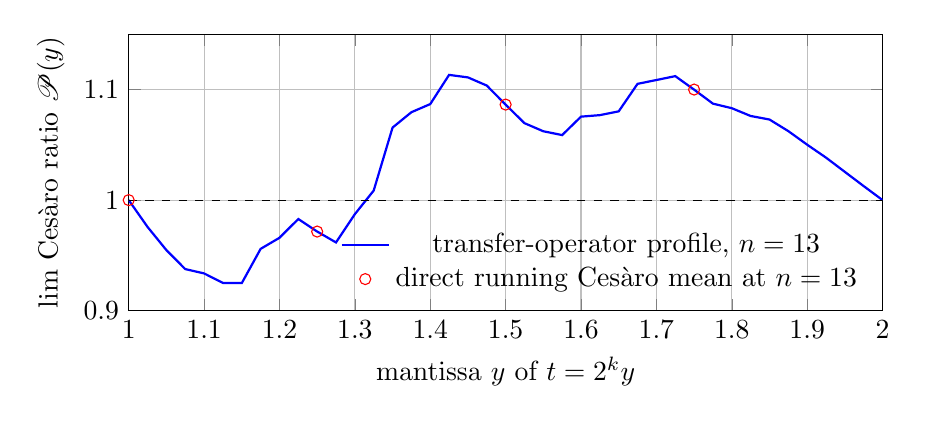
\begin{tikzpicture}
\begin{axis}[
 width=0.92\textwidth, height=0.42\textwidth,
 xlabel={mantissa $y$ of $t=2^ky$},
 ylabel={$\lim$ Ces\`aro ratio $\mathscr P(y)$},
 xmin=1, xmax=2, ymin=0.90, ymax=1.15,
 grid=major,
 legend style={at={(0.985,0.03)},anchor=south east,draw=none,fill=none},
]
\addplot+[mark=none, thick] coordinates {
(1.000,1.000000) (1.025,0.975728) (1.050,0.954767) (1.075,0.937622)
(1.100,0.933706) (1.125,0.925107) (1.150,0.924945) (1.175,0.955916)
(1.200,0.965927) (1.225,0.982913) (1.250,0.971581) (1.275,0.961711)
(1.300,0.987308) (1.325,1.008666) (1.350,1.065581) (1.375,1.079491)
(1.400,1.086830) (1.425,1.113237) (1.450,1.110962) (1.475,1.103570)
(1.500,1.086317) (1.525,1.069579) (1.550,1.062241) (1.575,1.058815)
(1.600,1.075481) (1.625,1.076833) (1.650,1.080254) (1.675,1.105143)
(1.700,1.108589) (1.725,1.112109) (1.750,1.099910) (1.775,1.087225)
(1.800,1.083115) (1.825,1.076078) (1.850,1.072880) (1.875,1.062386)
(1.900,1.050114) (1.925,1.038413) (1.950,1.025519) (1.975,1.012655)
(2.000,1.000000)
};
\addlegendentry{transfer-operator profile, $n=13$}
\addplot+[only marks, mark=o] coordinates {
(1.25,0.971559) (1.50,1.086373) (1.75,1.099966) (1.0,1.000000)
};
\addlegendentry{direct running Ces\`aro mean at $n=13$}
\addplot[dashed] coordinates {(1,1) (2,1)};
\end{axis}
\end{tikzpicture}
\caption{The dyadic-mantissa profile obstructing \eqref{eq:Q2}: the limit
of the Ces\`aro ratio at $t=2^ky$ as a function of $y$, for the normalized
gauge $A_1g_1$.  The curve is the transfer-operator prediction (partial
$P_{13}$-mass distribution); the circles are wholly independent running
Ces\`aro means over $[8,2^{13}y]$ computed by direct quadrature of $|f|$.
The sharp mass accretion around $y=4/3$ reflects the concentration of
the eigenmeasure near the preimages of the Gelfond-maximizing cycle
$\{1/3,2/3\}$.}
\label{fig:profile}
\end{figure}

\section{Interpretation in detail, I: the envelope of the lobe maxima}
\label{sec:lobes}

The zeros of $f$ at the integers divide $(0,\infty)$ into unit lobes, and
$|f|$ has exactly one maximum
\[
 E_n=\max_{n\le x\le n+1}|f(x)|=|f(\xi_n)|,
 \qquad \xi_n\in(n,n+1),
\]
per lobe, with signed value $(-1)^{s_2(n)}E_n$ (audited; the sign law is
also the Atlas's ``sign of the Fabius sinc product'').  Reading the
question as ``find the envelope of the sequence $E_n$'' is natural --- it
is literally the subject of the companion question \cite{mse-extrema} ---
and this section shows exactly how far that reading can be pushed.  The
outcome is structural: \emph{the peak sequence reproduces the whole decay
spectrum of \cref{sec:interpretations} in miniature}, so it has a sharp
limsup envelope, a zero liminf on that envelope's scale, a Ces\`aro
envelope with the same exponent $\kappa_1$ as $|f|$ itself, and a
density-one law with the typical exponent $\kappa_0$ --- but no single
envelope.

\subsection{Geometry of one lobe, and a peak--integral comparison}

Two audited facts anchor everything: away from the integers
\begin{equation}
 (\log|f|)'(x)=-2x\sum_{k\ge1}\frac{1+\vtwo(k)}{k^2-x^2},
 \qquad
 (\log|f|)''(x)=-2\sum_{k\ge1}(1+\vtwo(k))\frac{k^2+x^2}{(k^2-x^2)^2}<0,
 \label{eq:lobe-derivatives}
\end{equation}
so every lobe of $|f|$ is strictly log-concave with a unique peak.  The
following comparison is the workhorse of the mean layer; it does not
appear in any of the four documents.

\begin{lemma}[peak--integral comparison]
\label[lemma]{lem:peak-integral}
There is an absolute constant $C$ such that for all $n\ge2$,
\[
 \int_n^{n+1}|f|\;\le\;E_n\;\le\;C\,(1+\log n)^{3}\int_n^{n+1}|f|.
\]
\end{lemma}

\begin{proof}
The left inequality is trivial.  For the right one, write
$d_0=1+\vtwo(n)$, $d_1=1+\vtwo(n+1)$, $\delta_0=\xi_n-n$,
$\delta_1=n+1-\xi_n$, and note $d_0,d_1\le1+\log_2(n+1)$.  Splitting off
the $k=n$ and $k=n+1$ terms of \eqref{eq:lobe-derivatives} and bounding
the rest crudely ($|k^2-x^2|\ge|k-x|\,n$ for $k\le2n$, quadratic tail
beyond, $1+\vtwo(k)\le1+\log_2k$) gives, for $x$ in the middle segment
$[n+\delta_0/2,\,n+1-\delta_1/2]$,
\[
 (\log|f|)'(x)=\frac{d_0}{x-n}\theta_0(x)-\frac{d_1}{n+1-x}\theta_1(x)
 +\bigO(\log^2n),
 \qquad
 \theta_i(x)\in[\tfrac9{10},\tfrac65],
\]
and
\[
 \bigl|(\log|f|)''(x)\bigr|
 \le\frac{3d_0}{(x-n)^2}+\frac{3d_1}{(n+1-x)^2}+C\log n .
\]
At the peak the derivative vanishes; since one of $\delta_0,\delta_1$ is
at least $\tfrac12$, the vanishing forces the other to satisfy
$d_i/\delta_i\le C\log^2n$, whence
$\delta_{\min}\ge c/\log^2 n$ and, on the middle segment around
$\xi_n$, the curvature is at most $\Lambda\le C\log^5n$.  By
log-concavity, $|f(\xi_n\pm s)|\ge E_n\e^{-\Lambda s^2/2}\ge E_n/\e$ for
$s\le\min(\Lambda^{-1/2},\delta_{\min}/2)\ge c\,(1+\log n)^{-5/2}$, and
integrating over that subinterval gives
$\int_n^{n+1}|f|\ge c\,E_n(1+\log n)^{-5/2}$, which is stronger than
claimed.
\end{proof}

Numerically the comparison is far tamer than the worst-case bound: over
the shells $k=9$--$13$ the per-lobe ratio $E_n/\int_n^{n+1}|f|$ has
median $1.992$, and its maximum ($4.55$ at $k=9$, $5.93$ at $k=13$,
growing roughly linearly in $k$) is attained each time by the lobe
\emph{abutting} $2^{k+1}$, i.e.\ the lobe pressed against the
highest-multiplicity zero of the shell --- the same two-adic geometry as
the valleys.

\subsection{The peak sequence is the spectrum in miniature}

\begin{theorem}[four layers of the peak sequence]
\label{thm:peak-layers}
Let $\mathcal E(x)=\exp(-(\log x)^2/(2\log2))$.
\begin{enumerate}
\item \emph{Sharp upper envelope.}
$\limsup_{n\to\infty}\bigl(\log E_n+\tfrac{(\log n)^2}{2\log2}\bigr)/\log
n=-\kappa_\infty$, and no larger exponent works: the limsup is attained
along the lobes containing $2^k\cdot\tfrac43$ (equivalently
$2^k\cdot\tfrac23$).  At second order the annular maxima carry the
Lambert-$W$ correction of Documents 1--2, beginning
$-(\log\log x)^2/(2\log2)$.
\item \emph{Zero liminf on that scale.}
$\liminf E_n/\bigl(\mathcal E(n)n^{-\kappa_\infty}\bigr)=0$: along
$n=2^k$ (and $n=m2^k$, odd $m$) the peaks obey the two-adic law
$E_{m2^k}\sim\frac{H(1)|H(m)|}{\e(k+1)}(m2^k)^{-(k+1)}$, whose leading
quadratic coefficient $-1/\log2$ is twice the universal one.  Within the
shell $[2^k,2^{k+1})$ the deepest lobe observed is the one abutting
$2^{k+1}$ (zero multiplicity $k+2$; confirmed at $k\in\{9,11,13\}$ by
computing every lobe of the shell), with the lobe after $2^k$
(multiplicity $k+1$) its two-adic twin at the left edge; the two-adic
law itself is verified through $k=16$ (\cref{ssec:valleys}).
\item \emph{Mean layer: exponent $\kappa_1$ again.}  By
\cref{lem:peak-integral},
\[
 \int_{2^k}^{2^{k+1}}|f|\;\le\;\sum_{2^k\le n<2^{k+1}}E_n
 \;\le\;C\,k^{3}\int_{2^k}^{2^{k+1}}|f|,
\]
so the shell means of the peak sequence have the same power
$\kappa_1=2.748070\ldots$ as the shell means of $|f|$, and every
Ces\`aro-type statement of \cref{thm:audit-answer} transfers to the peak
sequence up to the polylogarithmic slack.  Numerically the slack is a
sharp constant: over $k=9,\dots,14$,
\[
 \frac{\sum_{2^k\le n<2^{k+1}}E_n}{\int_{2^k}^{2^{k+1}}|f|\,\dd x}
 =1.9238,\;1.9237,\;1.9237,\;1.9237,\;1.9237,\;1.9238\,(\pm3\cdot10^{-5}),
\]
supporting the conjecture that the ratio converges to a constant
$\Theta_{\mathrm{peak}}=1.92372(3)$; granting it, the peak sequence has
the Ces\`aro gauge $A_1^{\mathrm{peak}}\,x^{-\kappa_1}\mathcal E(x)$ with
$A_1^{\mathrm{peak}}=\Theta_{\mathrm{peak}}A_1=0.175569\ldots$
\item \emph{Typical layer: exponent $\kappa_0$.}  For every
$\varepsilon>0$,
\[
 \frac{1}{2^k}\,\#\Bigl\{2^k\le n<2^{k+1}:
 \Bigl|\log E_n+\frac{(\log n)^2}{2\log2}+\kappa_0\log n\Bigr|
 \le\varepsilon k\Bigr\}\longrightarrow1 .
\]
\end{enumerate}
\end{theorem}

\begin{proof}
(i) The upper bound is the uniform envelope (audited); sharpness is the
exact ray $y=4/3$.  (ii) is Documents 2 and 4's theorem (audited;
verified numerically with the slow $1/k$-type approach documented in
\cref{ssec:valleys}).  (iii) is immediate from \cref{lem:peak-integral}
after summing over the shell.  (iv) requires an argument, given now.

\emph{Lower half (few lobes are too small).}  Write $x=2^ky$,
$z=y-1$, so that by the factorization and the $\kappa$-algebra,
\[
 \log|f(x)|+\frac{(\log x)^2}{2\log2}+\kappa_0\log x
 =\Sigma_{k+1}(z)+\Psi(y),
 \qquad
 \Sigma_m(z):=\sum_{j=0}^{m-1}\psi(\T^jz),
\]
with $\psi=\log|2\sin\pi\cdot|$ centered and $\Psi$ bounded on
$[1,2)$.  By the Birkhoff theorem $\Sigma_m/m\to0$ a.e., hence in
measure: $\mathrm{Leb}\{z:|\Sigma_{k+1}(z)|>\tfrac\varepsilon2k\}\to0$.
A lobe occupies a $z$-cell of length $2^{-k}$; if the cell contains a
point of the good set, then $E_n\ge|f|$ there exceeds the
$\kappa_0$-line by more than $-\varepsilon k$.  The number of cells
disjoint from the good set is at most $2^k\cdot\mathrm{Leb}(\text{bad})
=\smallo(2^k)$.

\emph{Upper half (few lobes are too large).}  Call a cell $J$
\emph{regular} if for every $j\le k':=k-4\lceil\log_2k\rceil$ the image
$2^jJ$ keeps distance at least $k^2\,2^{j-k}$ from $\Z$.  For each $j$
the offending set is $2^j$ intervals of length $2k^22^{-k}$ each, so at
most $(2k^2+2)2^j$ cells are irregular at level $j$, and summing over
$j\le k'$ gives at most $C2^k/k^2=\smallo(2^k)$ irregular cells.  On a
regular cell every retained factor has logarithmic oscillation at most
$\pi/k^2$ across the cell (length times $\pi2^j\cot$-bound), so
\[
 \max_{J}P_{k+1}\le\e^{\pi/k}\,P_{k'}(z_J)
 \qquad\text{for every } z_J\in J,
\]
after discarding the last $4\lceil\log_2k\rceil$ factors, each bounded by
one.  Now fix $\varepsilon$ and choose $q\in(0,1)$ with
$\log\varrho_q<-q(1-\tfrac\varepsilon2)\log2$, possible because
$(\log\varrho_q)/(q\log2)\to-1$ as $q\downarrow0$ (the pressure slope at
the Lebesgue equilibrium; with the RPF package for $\Lop_q$ on
bounded-variation functions --- the weights $s^q$ have total variation
$2$ uniformly in $q\in[0,1]$ --- this is standard perturbation theory,
and it is the one imported input here, the same package as
\cref{ssec:imported}).  Markov's inequality with
$I_q(k')\le C_q\varrho_q^{k'}$ then bounds the measure of
$\{P_{k'}\ge\e^{-(1-\varepsilon)k\log2}\}$ by $\e^{-c(\varepsilon)k}$;
since on a regular cell all points give comparable $P_{k'}$, the number
of regular cells whose maximum exceeds the threshold is
$2^k\e^{-c(\varepsilon)k}=\smallo(2^k)$.  For such good cells,
$E_n\le C\cdot\text{shell factor}\cdot\e^{-(1-\varepsilon)k\log2}$ lies
below the $\kappa_0$-line by at most $\varepsilon k\log 2+\bigO(\log k)$.
Adjusting $\varepsilon$ absorbs the constants.
\end{proof}

\begin{proposition}[central limit law for the peaks]
\label[proposition]{prop:peak-clt}
For every $u\in\R$,
\[
 \frac{1}{2^k}\,\#\Bigl\{2^k\le n<2^{k+1}:
 \log E_n+\frac{(\log n)^2}{2\log2}+\kappa_0\log n
 \le u\,\frac{\pi}{2}\sqrt{k}\Bigr\}
 \longrightarrow\Phi(u),
\]
where $\Phi$ is the standard normal distribution function.
\end{proposition}

\begin{proof}
All ingredients are already on the table.  The continuous CLT
$\Sigma_k/\sqrt k\Rightarrow\mathcal N(0,\pi^2/4)$ holds by Document 1's
martingale argument with the variance of \cref{thm:variance}.
Convergence in distribution under Lebesgue measure transfers to the cell
ensemble because, outside the $\smallo(2^k)$ irregular cells, all points
of a cell give the same $\Sigma_{k'}$ up to $\pi/k$, and the discarded
top factors change $\log E_n$ by at most $\bigO(\log^2k)$ in one
direction and, in the other, by at least $\log$ of the product of the
discarded factors on a nested subcell: choosing inside the cell,
factor by factor from the finest down, the third of the current subcell
on which the new factor exceeds $\tfrac12$ leaves a nonempty subcell on
which the discarded product is at least $2^{-4\lceil\log_2k\rceil}$.
Both corrections are $\bigO(\log^2 k)=\smallo(\sqrt k)$, as is the
bounded mantissa term, so the cell statistics of $\log E_n$ inherit the
Gaussian limit with the same normalization.
\end{proof}

The measured quantiles agree on the left and are compressed on the
right, exactly as they must be at finite $k$: standardized quantiles at
$k=13$ are
$(-1.63,-0.43,+0.05,+0.36,+0.65)$ at levels
$(5,25,50,75,95)\%$ against the Gaussian
$(-1.645,-0.674,0,+0.674,+1.645)$.  The median sits on the
$\kappa_0$-line to within $0.05$ standard units --- the typical exponent
is visibly $\kappa_0$ --- while the right tail is truncated by the
deterministic Gelfond cap: no peak can exceed the $\kappa_\infty$-line,
which sits only
$(\kappa_0-\kappa_\infty)\log2\cdot\sqrt k/(\pi/2)\approx0.35\sqrt k$
standard units above the center ($\approx1.26$ at $k=13$).  The
truncation recedes like $\sqrt k$, so the Gaussian limit opens up only
logarithmically slowly in $x$ --- the same finite-size phenomenon that
hides the LIL constant from small-$L$ simulations in \cref{sec:lil}.

\subsection{The discrete dictionary: peaks as Thue--Morse spectra}

Across the shell $[2^k,2^{k+1})$, the lobe of $n=2^k+m$ occupies the
$z$-cell of $m2^{-k}$, and up to the bounded factors above,
$E_n$ is the windowed maximum of $P_{k+1}$ there --- that is, of the
modulus of the Thue--Morse polynomial
$\sum_{r<2^{k+1}}(-1)^{s_2(r)}\e^{2\pi\ii rz}$ near the dyadic frequency
$m/2^k$.  The peak-envelope interpretation is thus exactly the question
of the value distribution of Thue--Morse spectra, and the exact grid
identities of that world transfer:

\begin{proposition}[two exact grid identities]
\label[proposition]{prop:grid}
For every $n\ge1$:
\[
 \text{(i)}\quad
 \prod_{r=1}^{2^n-1}2\sin\frac{\pi r}{2^n}=2^n,
 \qquad\qquad
 \text{(ii)}\quad
 \sum_{m=0}^{2^n-1}P_n\Bigl(\frac{m}{2^n}\Bigr)^2=1 .
\]
\end{proposition}

\begin{proof}
(i) is the classical evaluation $\prod_{r=1}^{N-1}(1-\omega^r)=N$ for
$\omega=\e^{2\pi\ii/N}$, taken in modulus.  It says that the mean of
$\psi=\log|2\sin\pi\cdot|$ over the \emph{nonzero} points of the
$2^n$-grid is $2^{-n}\log2^n\to0$ --- the grid analogue of
$\int_0^1\psi=0$, which is what makes the discrete Birkhoff sums behave
like the continuous ones.
(ii) Let $p(t)=\prod_{j<n}(1-\e^{2\pi\ii2^jt})$, of degree $2^n-1$ with
coefficients $\pm1$, so $|p|=2^nP_n$.  The $2^n$-point discrete
Parseval identity gives
$2^{-n}\sum_m|p(m/2^n)|^2=\sum_r|c_r|^2=2^n$, i.e.\
$\sum_mP_n(m/2^n)^2=1$.  (Verified to $10^{-12}$ at $n=6,10,14$; even
$m$ contribute exactly zero.)
\end{proof}

Identity (ii) is the discrete twin of $\int_0^1P_n^2=2^{-n}$: the
$q=2$ layer is rigid in both the continuous and the sampled world, a
point taken up in \cref{sec:rms}.

\subsection{Verdict for this interpretation}

No function $G$ satisfies $E_n/G(n)\to c>0$: the four layers of
\cref{thm:peak-layers} are separated by genuine powers of $x$, and even
within one layer the fluctuations are of iterated-logarithm size.  What
the interpretation \emph{does} admit is exactly what \eqref{eq:Q2}--%
\eqref{eq:Q3} admit for $|f|$: a bounded Ces\`aro normalization with the
same exponent $\kappa_1$ (via \cref{lem:peak-integral}), with the
empirical constant $\Theta_{\mathrm{peak}}=1.9237$ tying the two
readings together.  For the companion question \cite{mse-extrema}, the
sharp answers are the limsup envelope
$x^{-\kappa_\infty}\mathcal E(x)$ and the typical law
$x^{-\kappa_0+\smallo(1)}\mathcal E(x)$ --- two different formulas,
necessarily.

\section{Interpretation in detail, II: the root-mean-square amplitude}
\label{sec:rms}

The RMS reading asks for $g$ such that the quadratic Ces\`aro mean of
$(f/g)^2$ is tame.  Because $f=\widehat\Up$, the shell RMS of $f$ is the
energy spectral envelope of the up-function, and this is the one reading
in which the deleted draft's exponent $\log_2(2\pi)$ is correct.  It is
also, by a wide margin, the most rigid layer of the whole problem: its
per-level mean is exact, its subleading spectrum is computable in closed
form, and its envelope constant converges at a clean geometric rate with
alternating sign.

\subsection{Exactness at every scale}

The continuous identity $\int_0^1P_n^2=2^{-n}$ (\cref{prop:L2}) and the
discrete identity $\sum_mP_n(m/2^n)^2=1$ (\cref{prop:grid}) leave no
asymptotics in the $q=2$ numerator: both the Lebesgue mean and the
grid mean of $P_n^2$ equal $2^{-n}$ exactly, for every $n$.  All
remaining structure sits in the bounded mantissa weight, and it too is
spectrally transparent:

\begin{proposition}[exact subleading spectrum of $\Lop_2$]
\label[proposition]{prop:L2-spectrum}
The operator
$(\Lop_2h)(x)=\tfrac12[\sin^2(\tfrac{\pi x}2)h(\tfrac x2)
+\cos^2(\tfrac{\pi x}2)h(\tfrac{x+1}2)]$ satisfies, exactly,
\[
 \Lop_2\mathbf 1=\tfrac12\,\mathbf 1,
 \qquad
 \Lop_2\bigl[\sin2\pi x\bigr]=-\tfrac14\sin2\pi x,
 \qquad
 \Lop_2\bigl[1+3\cos2\pi x\bigr]=-\tfrac14\bigl(1+3\cos2\pi x\bigr),
\]
and on even Fourier modes it acts by frequency halving,
$\Lop_2\e^{2\pi\ii\,2m x}\mapsto\tfrac12\e^{2\pi\ii mx}$.
\end{proposition}

\begin{proof}
With $e_m(x)=\e^{2\pi\ii mx}$: for even frequency $2m$,
$\e^{2\pi\ii\,2m\frac{x}{2}}=e_m(x)$ on both branches and
$\sin^2+\cos^2=1$ gives $\Lop_2e_{2m}=\tfrac12e_m$ (the $m=0$ case is
the first display).  For $m=1$,
\[
 \Lop_2e_1
 =\tfrac12\e^{\pi\ii x}\bigl[\sin^2(\tfrac{\pi x}2)
 -\cos^2(\tfrac{\pi x}2)\bigr]
 =-\tfrac12\e^{\pi\ii x}\cos\pi x
 =-\tfrac14\bigl(e_1+\mathbf 1\bigr),
\]
and likewise $\Lop_2e_{-1}=-\tfrac14(e_{-1}+\mathbf1)$.  Hence
$\{\mathbf1,e_1,e_{-1}\}$ spans an invariant subspace on which $\Lop_2$
has matrix eigenvalues $\{\tfrac12,-\tfrac14,-\tfrac14\}$; the real
eigenfunctions for $-\tfrac14$ are
$\sin2\pi x=(e_1-e_{-1})/2\ii$ and $1+3\cos2\pi x$ (direct check:
$\Lop_2[3\cos2\pi x]=-\tfrac34(1+\cos2\pi x)$, so
$\Lop_2[1+3\cos]=\tfrac12-\tfrac34-\tfrac34\cos=-\tfrac14(1+3\cos)$).
\end{proof}

Collocation places the rest of the spectrum below $3\cdot10^{-4}$ in
modulus, so the shell-RMS ratios converge at the exact geometric rate
$\lambda_2/\lambda_1=-\tfrac12$ per shell --- relative error
$\bigO(1/x)$, with alternating sign.  This is visible to the eye in the
measurements: the shell means of $(f/g_{\kappa_2})^2$ for
$k=4,5,6,7,8$ differ from their limit by
$+1.51\cdot10^{-5}$, $-7.6\cdot10^{-6}$, $+3.8\cdot10^{-6}$,
$-1.9\cdot10^{-6}$, $+0.94\cdot10^{-6}$ --- each step multiplying the
error by $-\tfrac12$ to the displayed accuracy --- with limit
\[
 A_2^2=0.0106108372\ldots,
 \qquad
 A_2=0.103008918\ldots
\]
(direct quadrature and the spectral iteration agree; the $L^1$ layer,
by contrast, has the non-elementary subleading pair
$-0.13435\pm0.0500\ii$ of modulus $0.1434$, rate
$|\lambda_2|/\varrho_1=0.217$ per shell).

\subsection{The RMS answer to the averaged question}

\begin{theorem}[RMS version of \cref{thm:audit-answer}]
\label{thm:rms-answer}
Let $G_2=A_2\,x^{-\kappa_2}\mathcal E(x)$ with
$\kappa_2=\log_2(2\pi)$.  Then:
(i) the quadratic Ces\`aro ratio
$\frac1{t-t_0}\int_{t_0}^t(f/G_2)^2$ is eventually confined to a compact
subinterval of $(0,\infty)$ and tends to $1$ along $t=2^k$ with relative
error $\bigO(2^{-k})$;
(ii) for $t=2^ky$ with fixed $y\in(1,2)$ it converges to a continuous,
nonconstant mantissa profile $\mathscr P_2(y)$, so the limit for all
$t$ fails --- for the same reason as at $q=1$: the $\Lop_2$-eigenmeasure
$\nu_2$ is atomless and singular;
(iii) the logarithmic mean
$\frac1{\log(t/t_0)}\int_{t_0}^t(f/G_2)^2\,\frac{\dd x}{x}$ converges
for all $t\to\infty$.
\end{theorem}

\begin{proof}
(i) and (iii) are verbatim the proofs of
\cref{thm:audit-answer}(i)--(ii) and \cref{thm:logmean} with
$(P_n,\varrho_1,W)$ replaced by $(P_n^2,\tfrac12,W_2)$; the improved
rate in (i) is \cref{prop:L2-spectrum}.  For (ii), only the two measure
statements change.  \emph{Atomless:} the eigenmeasure equation gives
$\nu_2(\{\T z\})=\nu_2(\{z\})/\sin^2(\pi z)\ge\nu_2(\{z\})$, with
equality only at $z=\tfrac12$.  No forward orbit can linger where
$\sin^2$ is near $1$: if $w\in[\tfrac38,\tfrac58]$ then
$\T w\in[0,\tfrac14]\cup[\tfrac34,1]$, where $\sin^2\le\tfrac12$; and
off $[\tfrac38,\tfrac58]$ one has $\sin^2\le\sin^2(\tfrac{3\pi}8)<0.854$.
So along any orbit the atom mass is nondecreasing and gains a factor
$\ge1/0.854$ at least every second step, forcing it to zero whether the
orbit is eventually periodic (mass grows around each loop) or not
(infinitely many distinct atoms of nonvanishing mass).
\emph{Singular:} an absolutely continuous part would have density $r$
with $\sin^2(\pi z)\,r(\T z)=\tfrac12r(z)$, hence
$r(\T^nz)=2^{-n}r(z)/P_n(z)^2$; for a.e.\ $z$ the Birkhoff theorem
gives $P_n(z)^2=\e^{-2n\log2(1+\smallo(1))}$, so on $\{r>0\}$ the
density grows like $\e^{n(\log2+\smallo(1))}$, contradicting
$r\in L^1$ by the same Borel--Cantelli argument as before.  (The general
criterion behind both cases: the $q$-eigenmeasure is singular whenever
$\varrho_q\e^{q\log2}>1$, i.e.\ whenever $\kappa_q<\kappa_0$; at
$q=2$ this reads $\tfrac12\cdot4=2>1$.)  The nonconstancy of
$\mathscr P_2$ then follows as in \cref{thm:impossible}.
\end{proof}

The measured $L^2$ profile (same transfer computation as
\cref{fig:profile}, weight $W_2P_{13}^2$) spans
$[0.894,\,1.192]$ --- wider than the $L^1$ profile
$[0.925,\,1.113]$, as expected, since squaring weights the singular
concentration near the Gelfond preimages more heavily.  So even the most
rigid reading of the question keeps the dyadic phase obstruction; what
it gains is exact constants and an $\bigO(1/x)$ rate everywhere the
limit does exist.

\subsection{Plancherel, Poisson, and the total energy}

\begin{proposition}[total energy]
\label[proposition]{prop:energy}
\[
 \int_{\R}f(x)^2\dd x=\int_{\R}\Up(t)^2\dd t
 =\frac12+\sum_{m=0}^{\infty}f\Bigl(m+\frac12\Bigr)^{2}
 =0.808873535967972\ldots
\]
\end{proposition}

\begin{proof}
The first equality is Plancherel ($f=\widehat\Up$, real and even).  For
the second, expand $\Up$, supported in $[-1,1]$, in Fourier series on
$[-1,1]$: the coefficients are $\tfrac12\widehat\Up(k/2)=\tfrac12f(k/2)$,
and Parseval gives
$\int\Up^2=\tfrac12\sum_{k\in\Z}f(k/2)^2$; the even $k\ne0$ terms vanish
($f$ vanishes at nonzero integers), $k=0$ gives $\tfrac12$, and the odd
terms pair up.  Numerically the direct quadrature
$2\int_0^{2^{14}}f^2$ and the series agree to $2\cdot10^{-15}$, the
displayed value; the series converges with super-Gaussian speed since
$f(m+\tfrac12)^2$ decays like $\mathcal E(m)^2$.
\end{proof}

This is a satisfying exactness check on the entire numerical apparatus,
and a natural first formalization target on the $L^2$ side: the
ingredients (compact support, the sinc product, Parseval on an interval)
are all present in the Lean development
(\lean{FourierProduct}, \lean{PoissonSummation}).

\subsection{The lognormal fallacy, quantified}

Why did plausible heuristics --- the deleted draft included --- land on
wrong exponents?  Because every mean-type interpretation lives in the
large-deviation regime of the lacunary product, where the correct
generating function is the pressure $q\mapsto\log\varrho_q$, not the
CLT parabola.  The exact offset formula (immediate from the
definitions) is
\[
 \kappa_0-\kappa_q=1+\frac{\log\varrho_q}{q\log2},
\]
giving the exact value $\tfrac12$ at $q=2$; a lognormal extrapolation of
the CLT would instead predict
$\kappa_0-\kappa_q^{\mathrm{LN}}=q\sigma^2/(2\log2)$ with
$\sigma^2=\pi^2/4$.  The comparison:

\begin{center}
\small
\begin{tabular}{@{}rlll@{}}
\toprule
$q$ & $\varrho_q$ & $\kappa_q$ (true) & $\kappa_q^{\mathrm{LN}}$
(lognormal)\\
\midrule
$0.25$ & $0.872813205188$ & $2.936517$ & $2.706533$\\
$0.5$  & $0.786052008490$ & $2.846103$ & $2.261569$\\
$1$    & $0.661322602061$ & $2.748070$ & $1.371642$\\
$2$    & $0.5$ (exact)    & $2.651496$ & $-0.408211$\\
$4$    & $0.320194101601$ & $2.562241$ & $-3.967919$\\
$\infty$ & ---            & $2.359015$ & $-\infty$\\
\bottomrule
\end{tabular}
\end{center}

Already at $q=2$ the lognormal prediction is not merely off --- it is
negative, i.e.\ it predicts moment \emph{growth} relative to the
typical scale that the function cannot deliver: the deterministic
Gelfond cap $P_n\le C(\sqrt3/2)^n$ truncates the upper tail that a
lognormal law would need.  The pressure slope
$(\log\varrho_q)/(q\log2)$, measured as $-0.785$, $-0.695$,
$-0.597$ at $q=\tfrac14,\tfrac12,1$, bends away from its $q\to0$ limit
$-1$ immediately: the moments leave the Gaussian bulk at once.  Three
consequences deserve record.  First, the draft's exponent is exactly
the $q=2$ row --- a correct constant attached to the wrong norm.
Second, the draft's proposed $(\log x)^{-1/2}$ factor is refuted most
decisively in this, its most favorable, reading: the shell RMS
normalization converges to the \emph{constant} $A_2$ at a geometric
rate, so no logarithmic factor of any exponent survives.  Third, the
spacing of the four headline exponents
$\kappa_\infty<\kappa_2<\kappa_1<\kappa_0$ is itself the multifractal
signature of the dyadic dynamics; treating any one of them as ``the''
decay rate discards the others' regimes, which is precisely the
category error the original conjecture made.

\section{Audit of the four documents}
\label{sec:audit}

The four documents pairwise overlap heavily and agree on every overlapping
claim except one (the iterated-logarithm constant, \cref{sec:lil}).
Documents 1 and 2 analyze the pointwise, typical, and extremal regimes;
Documents 3 and 4 additionally analyze the mean regimes and are the only
two that answer the question actually asked.

\subsection{Document 1 (\emph{Decay of the Fourier Transform \dots:
Dyadic products, ergodic fluctuations, and sharp annular envelopes})}

\emph{Content.}  Exact dyadic decomposition; zero multiplicities and
Thue--Morse signs; one extremum per unit interval; typical-ray law with
$\kappa_{\mathrm{typ}}=\kappa_0$; a central limit theorem with per-step
variance $\pi^2/4$ via the martingale difference
$d=\log|\tan\pi x|$; a law of the iterated logarithm with constant
$(\pi/2)\sqrt{2N\log\log N}$; the maximal invariant average
$\beta=\log(\sqrt3/2)$ with the slow-ray exponent
$\kappa_*=\kappa_\infty$; and the annular maximum
$\log M_N=-\tfrac a2N^2+(\beta-\log\pi-\tfrac a2)N
-\frac{(\log N)^2}{2a}+\frac{\log N\log\log N}{a}+\bigO(\log N)$.

\emph{Verified.}  The exact decomposition (\cref{sec:core}); the algebra of
its centered form (resymbolized independently); $\kappa_0$, $\kappa_*$ to
all printed digits; the variance $\pi^2/4$ and covariances
$\pi^2/(12\cdot2^k)$ (Monte Carlo and quadrature,
\cref{ssec:variance}); $\int_0^1\log^2|\tan\pi x|\dd x=\pi^2/4$;
$Pd=0$; the Green--Kubo resummation $\pi^2/12+2\sum_k\pi^2/(12\cdot2^k)
=\pi^2/4$ in its appendix; the annular expansion's first three terms agree
with Document 2's Lambert form after expanding $W$.

\emph{Defects.}
(i) \textbf{Scope}: the document never addresses the Ces\`aro question
\eqref{eq:Q2}--\eqref{eq:Q3}; its conclusions answer the deleted draft's
pointwise claim instead of the Stack Exchange question.  Within the
question's actual reading it is a (high-quality) analysis of the wrong
functional.
(ii) The boundary-layer theorem's error term $\bigO(\log N)$ is coarser
than Document 2's $\bigO((\log\log N)^2)$; not an error, but strictly
subsumed.
(iii) No numerical validation is supplied; all of its constants
nevertheless survived this audit's numerics.  Notably, its fluctuation
section is the one place in the entire corpus that contradicts---and,
as \cref{sec:lil} shows, corrects---the published literature.

\subsection{Document 2 (\emph{Sharp Real-Axis Decay \dots: Lambert $W$
boundary layers, and two-adic troughs})}

\emph{Content.}  Everything in Document 1's extremal track, sharpened: the
annular maximum in closed Lambert form,
\[
 \log M_k=-\tfrac{\lambda}{2}k(k+1)-(k{+}1)\log\pi+(k{+}1)\beta
 -\frac{W(c(k{+}1))^2+2W(c(k{+}1))}{2\lambda}
 +\bigO\bigl((\log\log k)^2\bigr),
 \quad c=\tfrac{\lambda}{\pi}\sqrt{\tfrac32},
\]
an elementary sharp Gelfond bound
$Q_n\le\sqrt{5/3}\,(\sqrt3/2)^n$ via an explicit algebraic subaction,
two-adic trough asymptotics
$E_{m2^k}\sim\frac{H(1)|H(m)|}{\e(k+1)}(m2^k)^{-(k+1)}$ for odd $m$, a
numerical table of $\log M_k$, and---critically---an explicit section
stating that the Ces\`aro question is a \emph{different}, $L^1$,
transfer-operator problem which the document does not solve.

\emph{Verified.}  The subaction identity
$3V(u)-4uV(4u(1-u))=\tfrac{(2u+1)(4u-3)^2}{3}$, $V(u)=1+\tfrac23u$
(expanded symbolically: exact); the annular table: this audit's independent
maximization reproduces all ten rows of its $(\log M_k,\;x^*/2^k)$ table to
every printed digit ($10^{-6}$), $k=3,\dots,12$ (\cref{ssec:maxima});
$H(1)=0.55377127588881009534\ldots$ (recomputed to 30 digits, matches all
20 printed); the Lambert residuals (bounded, $-0.72$ to $-0.82$, consistent
with the claimed $\bigO((\log\log k)^2)$ window); the trough law for
$m=1$ and $m=3$ (\cref{ssec:valleys}); the predicted drift of the annular
maximizer from mantissa $7/6$ toward deeper preimages of $1/3$ --- observed
exactly at $k=14$, where the maximizer jumps from
$x^*/2^k\approx1.16667$ to $\approx1.08333=13/12$.

\emph{Defects.}
(i) Scope: same as Document 1, but self-aware --- its \S9 correctly
scopes the Ces\`aro problem to the transfer-operator framework that
Documents 3 and 4 then execute; among the four only Document 2 draws this
boundary explicitly.
(ii) The two-adic trough asymptotic converges slowly; at $k=16$ the
measured $\log E_{2^k}$ still exceeds the limit formula by $0.098$
(a $10\%$ multiplicative residual, decaying roughly like $1/k$).  The
statement is asymptotically consistent but numerically ``young'' at
accessible $k$; a one-line remark on the convergence speed would have
prevented over-reading.
(iii) No fluctuation theory (deliberate).

\subsection{Document 3 (\emph{Sharp Decay Laws \dots: extremal envelopes,
metric fluctuations, and Ces\`aro normalization})}

\emph{Content.}  The widest scope: exact factorization; typical law;
one-sided iterated-logarithm fluctuations (quoted from \cite{ahl2017});
extremal envelope with an elegant ergodic-optimization proof (pushforward
to the logistic map, inequality $z^3(1-z)\le27/256$); the $L^1$ theory:
Fouvry--Mauduit asymptotic, transfer operator \eqref{eq:L1},
$\lambda=0.661322602060565$, $\beta_1=\kappa_1$, an explicit gauge, the
bounded-Ces\`aro theorem, the dyadic-endpoint limit, and the
singular-eigenmeasure obstruction to \eqref{eq:Q2}; the exact $L^2$
identity and the identification of the deleted draft's exponent as
$\kappa_2$; the $L^p$ pressure spectrum with endpoints
$p\downarrow0$, $p\to\infty$; Chebyshev-collocation numerics.

\emph{Verified.}  The ergodic-optimization lemma (equality case included);
$\lambda$ to thirteen digits by two independent methods; $\kappa_1$
(the printed $2.748070014871334$ against this audit's
$2.748070014871335$ from $\varrho_1=0.661322602060565$: the discrepancy
is one unit in the last place, inside the $\pm5\cdot10^{-15}$ uncertainty
inherited from $\varrho_1$'s own last digit);
the collocation table (all displayed eigenvalues reproduced to
$10^{-15}$); $\kappa_1$ (its printed $2.748070014871334$ is exactly the
value of $\tfrac12+\log_2(\pi/\varrho_1)$ at
$\varrho_1=0.661322602060565$, recomputed here in 25-digit arithmetic);
the bounded-Ces\`aro theorem and the dyadic-endpoint limit
(measured, \cref{ssec:cesaro}); the singularity argument for the
equilibrium measure (checked line by line; the inequality
$\log\lambda>-\log2$ that it needs follows rigorously from
$\varrho_1\ge3^{-1/2}$, \cref{prop:bracket}); the Fouvry--Mauduit and
Aistleitner--Hofer--Larcher attributions (verbatim against the published
paper and the authors' arXiv source); the $L^2$ identity; the
identification $\tfrac12+\log_2(\pi\sqrt2)=\log_2(2\pi)$.

\emph{Defects.}
(i) \textbf{Its Theorem 4.2 (sharp upper metric fluctuation) states
$\limsup_nS_n(t)/\sqrt{n\log\log n}=\pi$ a.e.}  The quotation is a
\emph{faithful} rendering of the published Theorem 1.2 of \cite{ahl2017},
but the published constant is itself erroneous by a factor $\sqrt2$; the
correct value is $\pi/\sqrt2$ (\cref{sec:lil}).  Every restatement
downstream (its (LIL-$x$) display and the abstract's
``excursion'' constant) inherits the factor.  The \emph{order}
$\sqrt{\log\xi\,\log\log\log\xi}$, and every conclusion drawn from it
(no fixed power of $\log x$ can flatten the amplitude), are unaffected.
(ii) Minor: the claim that its gauge has ``eventually monotone
derivatives of any order'' is proved per order (thresholds $X_m$ growing
with $m$); this matches the question's wording but is worth stating as
such, since no common half-line works for all orders simultaneously.

\subsection{Document 4 (\emph{Decay \dots: Dyadic renormalization,
transfer-operator norms, sharp envelopes, and exceptional valleys})}

\emph{Content.}  The most systematic mean-theory: a master normalization
identity; the full $L^q$ shell spectrum with monotonicity; exact
shell-geometric-mean constancy at $q=0$; the RMS row by Parseval; the
$q=1$ row with a \emph{rigorous, executable} Collatz--Wielandt/Sturm
certificate for $\varrho_1$; the same two-part Ces\`aro conclusion as
Document 3, but with complete proofs of the eigenmeasure's atomlessness
and singularity; a sharp two-step logarithmic inequality yielding the
Gelfond bound; a dyadic-boundary identity giving valley asymptotics for
every fixed offset $r$ (with the zero-multiplicity $d=1+\vtwo(r+1)$
appearing as the power of $1/n$); a continuum of intermediate quadratic
rates; and collocation numerics for $q\in\{1,2,3,4,8,16\}$.

\emph{Verified.}  The master identity (numerically exact); the $q=0$
exactness argument (each $j\ge1$ level integrates to $-\log2$ exactly on
the shell); the two-step inequality (cubed form reduces to
$\max u^3(1-u)=27/256$: exact); the atomlessness and singularity proofs
(sound; the Borel--Cantelli step uses only $T$-invariance of Lebesgue);
$\varrho_3=0.394896632370234$, $\varrho_4=0.320194101601104$ (matching
its table); \textbf{the certificate: executed verbatim under SymPy,
all four Sturm root-counts return zero and the assertions pass, so}
$0.66126807<\varrho_1<0.66134891$ \textbf{holds with exact rational
arithmetic}; the valley theorem for $r=0$ (equivalent to Document 2's
$m=1$ trough law; same slow convergence); the phase-profile formula
$\mathscr P(y)=(1+\mathscr F(2y-1))/(2y)$, realized numerically in
\cref{fig:profile}.

\emph{Defects.}
(i) No fluctuation theory at all: between the a.e.\ law ($q=0$ row) and
the shell means there is no CLT/LIL layer; Document 4 is silent exactly
where Documents 1 and 3 collide.  Since that collision is the corpus's
one real error surface, the omission kept Document 4 clean but also
unhelpful for adjudication.
(ii) Its Perron--Frobenius proposition asserts a spectral gap on
H\"older spaces for weights vanishing at the endpoints with a citation
rather than a proof; standard, but it is the one analytic ingredient of
its Ces\`aro theorem not reproved from scratch in any of the four
documents.
(iii) The ``intermediate rates'' section (quadratic coefficients
$-(1-\alpha+\alpha^2/2)/a$) is explicitly conditional on a typical-decay
hypothesis along the moving offset; it is a heuristic bridge, correctly
flagged as such, and was not counted as a theorem in this audit.

\subsection{Relations among the documents}

Document 1 $\subset$ Document 2 (extremal track, where 2 is sharper);
Documents 3 $\approx$ 4 (mean track, where 4 is more rigorous on $q=1$
and 3 is broader in scope).  The intersection of all four is the exact
factorization, $\kappa_0$, $\kappa_\infty$, and the refutation of the
deleted draft's pointwise claim.  The union, minus Document 3's inherited
LIL constant, plus the logarithmic-mean repair of
\cref{thm:audit-answer}(iv), is --- to the best of this audit's
verification --- a correct and essentially complete account of the
problem.

\section{The iterated-logarithm conflict and an error in the published
literature}
\label{sec:lil}

\subsection{The conflict}

For $S_L(t)=\sum_{j=0}^{L-1}\log|2\sin(\pi2^jt)|$:
\begin{itemize}
\item Document 1 proves a CLT with per-step variance $\pi^2/4$
(martingale differences $d=\log|\tan\pi x|$, $\int d^2=\pi^2/4$,
transfer-annihilation $Pd=0$) and the LIL
\[
 \limsup_{N}\frac{S_N}{\sqrt{2N\log\log N}}=\frac\pi2
 \quad\text{a.e., i.e.}\quad
 \limsup_{N}\frac{S_N}{\sqrt{N\log\log N}}=\frac{\pi}{\sqrt2}
 =2.2214\ldots
\]
\item Document 3 quotes the published Theorem 1.2 of \cite{ahl2017}:
for a.e.\ $\alpha$,
$\prod_{\ell=0}^{L}|2\sin\pi2^\ell\alpha|
\le\exp((\pi+\varepsilon)\sqrt{L\log\log L})$ eventually and
$\ge\exp((\pi-\varepsilon)\sqrt{L\log\log L})$ infinitely often ---
constant $\pi=3.1415\ldots$
\end{itemize}
These differ by exactly $\sqrt2$ and cannot both be sharp.

\subsection{The rigorous adjudication}

The conflict is decided by computing the variance exactly.  Write
$\psi(x)=\log|2\sin\pi x|$, $S_m=\sum_{\ell=0}^{m-1}\psi\circ\T^\ell$.

\begin{theorem}[exact variance of the lacunary sums]
\label{thm:variance}
$\psi\in L^2(0,1)$ with mean zero, and for every $m\ge1$,
\begin{equation}
 \int_0^1S_m(x)^2\dd x
 =\frac{\pi^2}{4}\,m-\frac{\pi^2}{3}\bigl(1-2^{-m}\bigr).
 \label{eq:exact-variance}
\end{equation}
In particular the functional (2.9) of \cite{ahl2017} evaluates, for
$f_1=\psi$, to
\[
 \sigma_{f_1}^2
 =\lim_{m\to\infty}\frac1m\int_0^1S_m^2
 =\frac{\pi^2}{4},
 \qquad\text{hence}\qquad
 \sigma_{f_1}=\frac{\pi}{2}.
\]
\end{theorem}

\begin{proof}
The Clausen expansion
$\psi(x)=-\sum_{j\ge1}\cos(2\pi jx)/j$ holds in $L^2(0,1)$ (the
coefficients are square-summable, and the series is the classical
Fourier series of $\psi$).  By Parseval, using
$\int_0^1\cos^2(2\pi jx)\dd x=\tfrac12$,
\[
 c_0:=\int_0^1\psi^2=\frac12\sum_{j\ge1}\frac1{j^2}=\frac{\pi^2}{12},
\]
and for $r\ge1$, since
$\int_0^1\cos(2\pi jx)\cos(2\pi k2^rx)\dd x=\tfrac12\,
\mathbf 1_{\{j=2^rk\}}$,
\[
 c_r:=\int_0^1\psi(x)\,\psi(2^rx\bmod1)\dd x
 =\frac12\sum_{k\ge1}\frac{1}{2^rk}\cdot\frac1k
 =\frac{\pi^2}{12}\,2^{-r}.
\]
Stationarity of $(\psi\circ\T^\ell)$ under Lebesgue measure gives
$\int S_m^2=mc_0+2\sum_{r=1}^{m-1}(m-r)c_r$, and the elementary
summation $\sum_{r=1}^{m-1}(m-r)2^{-r}=m-2+2^{1-m}$ yields
\eqref{eq:exact-variance}.  (Check at $m=1$:
$\pi^2/4-\pi^2/6=\pi^2/12=c_0$.)
\end{proof}

\begin{theorem}[corrected sharp constant]
\label{thm:lil-correct}
For Lebesgue-almost every $\alpha$,
\[
 \limsup_{L\to\infty}
 \frac{S_L(\alpha)}{\sqrt{2L\log\log L}}=\frac{\pi}{2},
 \qquad\text{equivalently}\qquad
 \limsup_{L\to\infty}
 \frac{\log\prod_{\ell=0}^{L}|2\sin\pi2^\ell\alpha|}
 {\sqrt{L\log\log L}}
 =\frac{\pi}{\sqrt2}=2.2214\ldots
\]
\end{theorem}

\begin{proof}[Proof (audit of Document 1's argument, with the boundary
estimates completed)]
Set $d=2\psi-\psi\circ\T$.  The double-angle identity gives
$d(x)=\log|\tan\pi x|$, and
$\int_0^1d^2=\tfrac2\pi\int_0^{\pi/2}\log^2\tan u\,\dd u
=\tfrac2\pi\cdot\tfrac{\pi^3}{8}=\tfrac{\pi^2}{4}$.
The transfer operator $P$ of $\T$ (fiber average over the two preimages)
annihilates $d$:
$d(x/2)+d((x+1)/2)=\log|\tan\tfrac{\pi x}2\cdot\tan(\tfrac{\pi x}2
+\tfrac\pi2)|=\log1=0$.  Hence $(d\circ\T^\ell)_{\ell\ge0}$ is a
stationary ergodic sequence of reverse martingale differences with
respect to the decreasing filtration $(\T^{-\ell}\mathcal B)$, with
orthogonal increments
($\int(P^kd)\,d=0$ for $k\ge1$) and variance $\pi^2/4$; note this
matches \cref{thm:variance}, as it must, since telescoping gives the
exact identity
\[
 S_L=\sum_{\ell=0}^{L-1}d\circ\T^\ell-\psi+\psi\circ\T^{L}.
\]
The law of the iterated logarithm for stationary ergodic
square-integrable (reverse) martingale difference sequences
(Stout; Heyde--Scott; via Skorokhod embedding, whose time change has
almost-surely linear growth $T_L/L\to\E d^2$ by the ergodic theorem)
gives
$\limsup\bigl(\sum_{\ell<L}d\circ\T^\ell\bigr)/\sqrt{2L\log\log L}
=\sqrt{\E d^2}=\pi/2$ a.e.  The boundary terms are almost surely
$\smallo(\sqrt{L\log\log L})$: $\psi\le\log2$ above, while
$\mathrm{Leb}(\psi<-u)\le\tfrac2\pi\e^{-u}(1+\smallo(1))$ gives
$\sum_L\Prob(\psi\circ\T^L<-2\log L)<\infty$, so by Borel--Cantelli
$\psi(\T^L\alpha)\ge-2\log L$ eventually a.e.  The product form follows
by exponentiating and absorbing the index shift $L\mapsto L+1$.
\end{proof}

Independently of the martingale route, the constant $\pi$ is excluded by
the tail calculus that any LIL proof must supply: with variance
$\pi^2/4$, exceedance probabilities at threshold
$(\pi-\varepsilon)\sqrt{L\log\log L}$ are
$(\log L)^{-(\pi-\varepsilon)^2/(2\sigma^2)}=(\log L)^{-2+\smallo(1)}$
at Gaussian scale, and dyadic block maxima then have summable
probabilities, so by Borel--Cantelli the lower bound (1.7) of
\cite{ahl2017} cannot hold with the constant $\pi-\varepsilon$
infinitely often.

\subsection{The source of the error, located in the authors' own text}

Theorem 1.2 of \cite{ahl2017} (arXiv numbering: Theorem 2, label
\texttt{th\_theorem2} in the authors' source file, of which the
repository now holds a copy at
\nolinkurl{docs/papers/arXiv-1502.06738v2/Lacunary_products.tex}) is
derived in the paper's Section 4 from its Lemma 4.1,
\[
 \limsup_{L\to\infty}
 \frac{\sum_{\ell=0}^{L-1}f_1(2^\ell\alpha)}{\sqrt{2L\log\log L}}
 =\frac{\pi}{\sqrt2}
 \quad\text{a.e.},\qquad f_1(\alpha)=\log|2\sin\pi\alpha|,
\]
which rests on Fortet's classical sharp LIL (the paper's Lemma 2.6):
$\limsup S_L/\sqrt{2L\log\log L}=\sigma_f$ with $\sigma_f^2$ given by the
functional (2.9) evaluated in \cref{thm:variance}.  The paper
evaluates the functional in its equation (4.5):
\[
 \sigma_{f_1}^2
 =\sum_{j=1}^{\infty}\Bigl(\frac{1}{j^2}
 +2\sum_{r=1}^{\infty}\frac{1}{2^rj^2}\Bigr)
 =\frac{\pi^2}{2}.
 \tag{4.5}
\]
Comparing term by term with the proof of \cref{thm:variance}: the
displayed sum is exactly $2c_0+2\sum_r2c_r$, i.e.\ each Parseval factor
$\int\cos^2=\tfrac12$ has been replaced by $1$.  The correct value is
$\pi^2/4$; hence Lemma 4.1's constant is $\pi/2$, and Theorem 1.2's is
$\pi/\sqrt2$.  Two internal cross-checks against the paper itself:
its equation (1.13) states the classical i.i.d.\ benchmark
$\limsup|\sum\e^{2\pi\ii hX_k}|/\sqrt{2N\log\log N}=1/\sqrt2$
\emph{correctly} (variance $\tfrac12$ of a single harmonic retained), and
applying the (4.5)-style evaluation to the single harmonic
$f=\cos2\pi\alpha$ would give $\sigma^2=1$ and hence a Hadamard-lacunary
LIL constant $1$ in the $\sqrt{2L\log\log L}$ normalization,
contradicting the classical Erd\H os--G\'al value $1/\sqrt2$ which
Fortet's formula reproduces.  The error is therefore an isolated slip in
the evaluation (4.5), identical in the arXiv source and in the published
version; it is not an OCR artifact (checked against the publisher's PDF
page images and the authors' own \LaTeX{} source).

\subsection{Numerical corroboration}

Sampling the doubling map on exact rational orbits
$p\mapsto2p\bmod q$ (odd moduli $q\approx2^{61}$, uniform residues, so
no floating-point orbit corruption at any length) gives
\begin{center}
\begin{tabular}{@{}lrrr@{}}
\toprule
 & measured & \eqref{eq:exact-variance}, $\sigma^2=\pi^2/4$ &
 same with $\sigma^2=\pi^2/2$\\
\midrule
$\Var(S_{20})$, $4\cdot10^5$ samples & $45.66$ & $46.06$ & $92.12$\\
$\Var(S_{34})$, $4\cdot10^5$ samples & $80.41$ & $80.60$ & $161.20$\\
$\Var(S_{1000})$, $4\cdot10^6$ samples & $2459.5$ & $2464.1$ & $4928.2$\\
\bottomrule
\end{tabular}
\end{center}
The covariance $\int_0^1\psi(x)\psi(2x)\dd x$ was measured as
$0.4112311$ against $\pi^2/24=0.4112335$.  Tail frequencies at $L=1000$
track the $\sigma=\pi/2$ Gaussian branch from below (the distribution is
left-skewed at finite $L$) and sit far below the $\sigma=\pi/\sqrt2$
branch: at threshold $\pi\sqrt{L\log\log L}$ the measured frequency is
$5.2\cdot10^{-4}$, against $2.7\cdot10^{-3}$ for the $\pi/2$ branch and
$2.5\cdot10^{-2}$ for the branch the printed constant would require.
A structural curiosity uncovered along the way: at small $L$ (e.g.\
$L=40$) the upper tail is \emph{cut off} by the deterministic Gelfond cap
$S_L\le L\log\sqrt3+\bigO(1)$, which sits below the
$c=2.9$ threshold there; the LIL scale detaches from this cap only for
$L\gtrsim10^2$--$10^3$, which is why na\"ive small-$L$ simulations
cannot see the asymptotic constant at all, and why the corroboration
above was run at $L=1000$ on exact orbits.

\begin{finding}[erratum-level correction to \cite{ahl2017}]
\label[finding]{find:ahl}
In Aistleitner--Hofer--Larcher, Ann.\ Inst.\ Fourier 67 (2017) 637--687:
equation (4.5) should read $\sigma_{f_1}^2=\pi^2/4$; Lemma 4.1 should
read $\pi/2$ in place of $\pi/\sqrt2$; the constant $\pi$ in Theorem 1.2
(equations (1.6)--(1.7)) should be $\pi/\sqrt2=2.2214\ldots$; and the
constant $\pi/\sqrt{\log2}=3.7735\ldots$ in Theorem 1.1 (equations
(1.4)--(1.5)) should be $\pi/\sqrt{2\log2}=2.6682\ldots$.  The paper's
$\sigma_{f_2}^2=0$ (equation (4.6)), its Theorem 1.3 (whose exponent
involves only $\lambda$), and Lemma 5.1's enclosure for $\lambda$ are
unaffected.  The publisher's PDF (read as page images), the repository's
OCR copy, and the authors' own arXiv \LaTeX{} source
(\nolinkurl{docs/papers/arXiv-1502.06738v2/}, where the theorem is
numbered Theorem 2, as Document 3 cites it) all show the same formulas,
so this is not a transcription artifact of any copy.
Consequently Document 3's Theorem 4.2 constant $\pi$ must be read as
$\pi/\sqrt2$, and Document 1's fluctuation section is correct as written.
\end{finding}

\emph{Postscript: a corrected edition.}  Following this audit, the
repository owner prepared a corrected critical edition of the paper,
stored alongside the OCR transcription as
\nolinkurl{AIF_2017__67_2_637_0-corrected.tex}.  On the four loci of
\cref{find:ahl} it agrees with the audit exactly: (1.4)--(1.5) now read
$\pi/\sqrt{2\log2}$, (1.6)--(1.7) read $\pi/\sqrt2$, Lemma 4.1 reads
$\pi/2$, and (4.5)--(4.6) carry the Parseval factor $\tfrac12$
(yielding $\pi^2/4$ and $0$), with the downstream Section 4 displays
updated consistently --- checked here by search: no occurrence of the
erroneous constants survives anywhere in the edition.  The edition goes
substantially beyond this audit's scope: it repairs the near-resonance
step (3.8)--(3.10), whose printed form divides by a ceiling that can
vanish for admissible indices, via a bipartite maximum-degree-two
argument; enlarges Lemma 2.1's exponential-moment constant from
$2\pi^2/3$ to $\pi^2$ and propagates the coarse constants
$29\to30$, $30\to31$, $85\to88$; removes Theorem 2.5's inconsistent
evenness hypothesis; and corrects a Fourier-tail summation range in
Section 4 along with numerous Section 5--6 transcription-level defects.
The spot-checks performed for this audit all pass: the internal
arithmetic of the new (3.9)
($\|p\|_2^2\le\pi^2/12$ on the diagonal, $S_{\ell_1,\ell_2}\le
\pi^2/(2R)$ off it, and
$\pi^2/12+\pi^2/(2(q-1))\le\tfrac{\pi^2}{2}\tfrac{q}{q-1}$ for
$q>1$), its coherence with the enlarged Lemma 2.1 bound
$\exp(\pi^2\lambda^2Lq/(q-1))$ (the per-block factor
$4\lambda^2W_i\le2\pi^2\lambda^2|\Delta_i|\tfrac q{q-1}$ telescopes
correctly), and the final Section 4 conversions to
$\pi/\sqrt{2\log2}$.  The Section 5--6 repairs were not independently
re-derived here and rest on the edition's own validation.

The meta-lesson for this repository's methodology deserves a sentence:
the error was surfaced not by checking any single document against the
literature --- Document 3 \emph{matches} the literature --- but by
insisting that two independently produced documents agree with each
other, and then measuring the disputed quantity.  Faithful citation is
not correctness.

\section{Numerical experiments}
\label{sec:numerics}

All experiments evaluate $\log|f|$ by summing
$\log|{\sinc}|$ over levels $h\le\log_2(\pi x)+30$ with a quartic Taylor
tail (absolute error below $10^{-15}$), and integrate over unit lobes by
24-point Gauss--Legendre panels.  Scripts: \cref{app:scripts}.

\subsection{Shell means and the constant $A_1$}
\label{ssec:shells}

$\frac{1}{2^{n-1}}\int_{2^{n-1}}^{2^n}|f|/g_1$, by direct quadrature and,
independently, as $\varrho_1^{-n}\int_0^1\Lop_1^n(W)\,$ by collocation
($N=40$) with Clenshaw--Curtis integration:
\begin{center}
\small
\begin{tabular}{@{}rllll@{}}
\toprule
$n$ & 4 & 6 & 10 & 14 \\
\midrule
direct   & 0.0912636508 & 0.0912662060 & 0.0912661248 & 0.0912661241\\
spectral & 0.0912636508 & 0.0912662060 & 0.0912661248 & 0.0912661241\\
\bottomrule
\end{tabular}
\end{center}
The two computations agree to all ten digits at every $n$ (they share no
code path beyond the evaluation of $H$), and the spectral iteration
continues to $A_1=0.0912661241$ unchanged through $n=60$.  This
simultaneously validates the factorization \eqref{eq:factorization},
$\varrho_1$, $\kappa_1$, and the spectral-gap convergence claimed by
Documents 3 and 4.

\subsection{Ces\`aro means: dyadic convergence and the mantissa profile}
\label{ssec:cesaro}

Running means $\frac{1}{t-t_0}\int_{t_0}^{t}|f|/(A_1g_1)$, $t_0=8$:
\begin{center}
\small
\begin{tabular}{@{}rcccc@{}}
\toprule
$t=y\cdot2^n$ & $y=1$ & $y=1.25$ & $y=1.5$ & $y=1.75$\\
\midrule
$n=5$  & 0.999992 & 0.964484 & 1.103575 & 1.116546\\
$n=9$  & 1.000000 & 0.971221 & 1.087225 & 1.100810\\
$n=13$ & 1.000000 & 0.971559 & 1.086373 & 1.099966\\
transfer-operator limit & 1 & 0.971581 & 1.086317 & 1.099910\\
\bottomrule
\end{tabular}
\end{center}
The dyadic column locks to $1$; the non-dyadic columns converge to the
predicted profile values (agreement $2\cdot10^{-5}$ to $6\cdot10^{-5}$ at
$n=13$).  The full profile (\cref{fig:profile}) has range
$[0.9249,1.1133]$ on a step-$0.025$ grid.  This is the numerical content
of ``\eqref{eq:Q3} yes, \eqref{eq:Q2} no''.

\subsection{The logarithmic mean}
\label{ssec:logmean}

$\frac{1}{\log(t/t_0)}\int_{t_0}^{t}|f|/g_1\cdot x^{-1}\dd x$ at the same
mantissas:
\begin{center}
\small
\begin{tabular}{@{}rcccc@{}}
\toprule
 & $y=1$ & $y=1.25$ & $y=1.5$ & $y=1.75$\\
\midrule
$n=7$  & 0.093861 & 0.092490 & 0.095987 & 0.096493\\
$n=13$ & 0.093861 & 0.093287 & 0.094781 & 0.095032\\
\bottomrule
\end{tabular}
\end{center}
All columns approach the common constant $A_1^{\log}=0.0938610$, at the
expected $\bigO(1/\log t)$ rate; the dyadic column is already exact
because complete shells contribute equally.  This substantiates
\cref{thm:audit-answer}(iv).

\subsection{Annular maxima and the Lambert formula}
\label{ssec:maxima}

Independent maximization (coarse scan over all unit intervals, then
bounded refinement), against Document 2's table and its Lambert
approximation $\mathcal A_k$:
\begin{center}
\small
\begin{tabular}{@{}rrrrr@{}}
\toprule
$k$ & $\log M_k$ (this audit) & $x^*/2^k$ & Document 2 & residual to
$\mathcal A_k$\\
\midrule
3  & $-11.251778$ & 1.177288 & $-11.251778$ & $-0.823$\\
6  & $-25.991031$ & 1.165501 & $-25.991031$ & $-0.728$\\
9  & $-46.956338$ & 1.166810 & $-46.956338$ & $-0.723$\\
12 & $-74.157742$ & 1.166649 & $-74.157742$ & $-0.783$\\
13 & $-84.611550$ & 1.166676 & --- & $-0.814$\\
14 & $-95.727351$ & 1.083338 & --- & $-0.818$\\
15 & $-107.493236$ & 1.083331 & --- & $-0.784$\\
\bottomrule
\end{tabular}
\end{center}
Rows $3$--$12$ reproduce Document 2's table to every printed digit.  At
$k=14$ the maximizer leaves the mantissa $7/6$ (one doubling to the
Gelfond cycle) for $13/12$ (two doublings), exactly the pre-period growth
$r=\log_2k-\log_2\log k+\bigO(1)$ predicted by Documents 1 and 2; the
Lambert residual stays in a bounded band, consistent with the claimed
$\bigO((\log\log k)^2)$ remainder.

\subsection{Two-adic valleys}
\label{ssec:valleys}

Peak of $|f|$ on $(2^k,2^k+1)$ against
$\frac{H(1)^2}{\e(k+1)}2^{-k(k+1)}$
(Documents 2 and 4; $H(1)=0.5537712759$):
$\log$-differences $+0.137$ ($k=8$), $+0.122$ ($k=12$), $+0.098$
($k=16$), decaying roughly like $1/k$; peak locations
$0.8804,0.9180,0.9378$ against the predicted $1-1/(k+1)=
0.8889,0.9231,0.9412$.  For $m=3$: differences $+0.156$ ($k=6$) down to
$+0.124$ ($k=12$), with $|H(3)|=0.0462022991$.  The valley laws are
supported as stated (asymptotic, with slow $1/k$-type approach).

\subsection{Variance and tails}
\label{ssec:variance}

See the table in \cref{sec:lil}.  Method: exact doubling orbits on odd
moduli $q\in[2^{61},2^{62})$, $p$ uniform on $[1,q)$; each orbit step is
one integer shift-and-mod; $\sin$ is evaluated in double precision from
the exact rational.  This eliminates the two artifacts that invalidate
na\"ive double-precision simulation (orbit collapse after $\sim50$
doublings, and spurious exact zeros from short mantissas), both of which
were observed and diagnosed before switching to rational orbits.

\subsection{The $\varrho_1$ certificate}
\label{ssec:certificate}

Document 4's Appendix A script was executed verbatim (SymPy 1.14):
for both bracketing rational functions the numerator and denominator
Sturm root counts on $[0,1]$ are zero and the sign checks at $t=0$ pass,
certifying $0.66126807<\varrho_1<0.66134891$ in exact arithmetic,
hence $2.74801262<\kappa_1<2.74818899$.  This is the strongest
rigor statement about $\kappa_1$ in the corpus, and it is machine-checkable.

\subsection{Exact spot identities}

$I_2(n)=2^{-n}$ verified to $10^{-12}$ ($n=2,5,8,11$); the slow-ray
identity $|f(2^k\tfrac43)|=|f(\tfrac43)|(3\sqrt3/(8\pi))^k2^{-k(k+1)/2}$
verified to $10^{-14}$ ($k=6$); Document 4's peak-ray constant
$W_{\kappa_\infty}(2/3)=0.139129774734829$ reproduced to all digits and
its ray identity verified to $10^{-13}$ ($n=9$); the collocation
eigenvalues $\varrho_2=\tfrac12$ (exact to $10^{-15}$),
$\varrho_3,\varrho_4$ as printed in Document 4.

\section{Relation to the repository corpus}
\label{sec:corpus}

\subsection{The deleted draft}
\label{sec:draft}

The \emph{Decay rate conjecture} draft (removed from the working tree;
recover with
\lstinline[basicstyle=\ttfamily\footnotesize]|git show e1cdd6260:".../Decay rate conjecture.tex"|)
claimed
\[
 g(x)\approx x^{\log(2\pi)/\log2}(\log x)^{-1/2}
 \exp\Bigl\{\frac{(\log x)^2}{2\log2}\Bigr\},
 \qquad g(x)f(x)\sim\text{constant},
\]
after an opening that asserts the opposite sign for the logarithmic
power.  The audit confirms the four documents' unanimous verdict: the
pointwise claim is false on three independent grounds (integer zeros;
iterated-logarithm fluctuations on typical rays; two-adic valleys), no
power of $\log x$ appears in any of the correct mean normalizations, and
the draft's power of $x$ is exactly the RMS exponent $\kappa_2$ ---
a meaningful constant attached to the wrong norm.  The draft's own
derivation sketch (termwise summation of the $\log|{\sin}|$ Fourier
series) is precisely the step that erases the dyadic orbit structure;
Documents 3 and 4 show what that structure contributes: the difference
between $\kappa_2$ and each of $\kappa_1$, $\kappa_0$, $\kappa_\infty$.

\subsection{Ties to existing material}

The Thue--Morse Formula Atlas already contains the sign law
$\sgn f|_{(N,N+1)}=\varepsilon_N$, the finite Fourier product, the
Gelfond exponent section (the $L^\infty$ row of the present dictionary),
and---as the structural twin of the universal factor---the boundary
flatness theorem $\log E(t)=-\log^2(1/t)/(2\log2)+\bigO(\log(1/t))$ for
$E(t)=\prod_j(1-\e^{-2^jt})$, including the remark that a bounded
log-periodic fluctuation persists at the next order.  The mantissa
profile of \cref{fig:profile} is the exact analogue of that fluctuation
for the decay problem, with the new feature that here the fluctuation is
driven by a \emph{singular} measure.  On the Lean side,
\lean{FourierProduct}/\lean{PoissonSummation} already carry the product,
the scaling law, and rapid decay; \lean{FabiusLogSquaredAsymptotic} and
its neighbors carry the small-argument $-\log^2$ layer.

\subsection{Formalization targets, ordered by feasibility}

\begin{enumerate}
\item The exact factorization \eqref{eq:factorization} and the
$\kappa$-algebra: finite manipulation of already-formalized objects.
\item $I_2(n)=2^{-n}$: finite Parseval over the Thue--Morse block,
adjacent to \lean{ThueMorseBlockAlgebra}.
\item The Gelfond bound via Document 4's two-step inequality (a single
polynomial inequality, \lean{nlinarith} territory) or Document 2's
subaction identity (pure algebra).
\item The $\varrho_1$ enclosure via the Sturm certificate: rational
positivity on an interval; decidable, and the certificate is already
machine-readable.
\item The valley asymptotics (elementary boundary-maximum analysis).
\item The variance $\sigma^2=\pi^2/4$: Parseval for the Clausen series
of $\log|2\sin\pi x|$ plus the geometric covariance sum; would also
formally certify \cref{find:ahl}.
\item Hardest: Birkhoff/ergodic layers and the Perron--Frobenius gap;
import as named hypotheses first, as Documents 3 and 4 recommend.
\end{enumerate}

\section{Verdict}
\label{sec:verdict}

\begin{enumerate}
\item \textbf{On the question asked.}  The bounded form \eqref{eq:Q3} is
solved, constructively: $g=A_1g_1$ of \eqref{eq:gauge}.  The exact-limit
form \eqref{eq:Q2} is unattainable for any gauge in the natural
(shell-shape-stabilizing, in particular Hardy-field) class; it becomes
attainable along dyadic times, or exactly and for all times under the
logarithmic mean.  This composite answer --- not any single formula ---
is the correct resolution of \cite{mse-decay}; within it, the 2018
answer of Negometyanov (a truncated $q$-Pochhammer representation,
useful for bounded-range evaluation) contains no asymptotic law, as the
question's author already noted at the time.  The two readings the four
documents left underdeveloped are now treated in full: the lobe-maxima
envelope decomposes into the same four regimes and rejoins the
$\kappa_1$ gauge through the peak--integral comparison, with
$\Theta_{\mathrm{peak}}=1.9237$ tying the peak and integral readings
together (\cref{sec:lobes}); and the root-mean-square reading is exactly
solvable --- closed subleading eigenvalue $-\tfrac14$, alternating
$\bigO(1/x)$ convergence, total-energy identity --- yet still carries
the dyadic phase obstruction (\cref{sec:rms}).
\item \textbf{On the four documents.}  All are technically serious, and
their factual overlap survived every numerical test applied here, in
several cases to all printed digits.  Documents 3 and 4 answer the
question; Document 4 is the most rigorous where they overlap (its
$\varrho_1$ certificate passes exact-arithmetic execution); Document 2
is the sharpest on the extremal geometry (its numerics reproduce
exactly) and the only one to scope the problem honestly; Document 1 is
subsumed by Document 2 except for its fluctuation section --- which
turned out to be the corpus's single most valuable page.
\item \textbf{Errors found.}  One substantive: the constant $\pi$ in
Document 3's Theorem 4.2, inherited verbatim from Theorem 1.2 of the
published \cite{ahl2017}, whose own equation (4.5) drops a Parseval
factor $\tfrac12$; the correct constant is $\pi/\sqrt2$
(\cref{find:ahl}), as Document 1 states.  All other deviations found
were of scope, convergence-speed candor, or single-ulp arithmetic.
\item \textbf{Recommended dispositions.}  Absorb into the frontier
volume: the $\kappa_q$ dictionary with the certificate-backed $q=1$ row;
the two-part answer to \eqref{eq:Q2}/\eqref{eq:Q3} with the mantissa
profile; the corrected fluctuation constants; the Lambert-form annular
envelope and valley laws with explicit convergence-speed caveats.
Annotate the OCR copy of \cite{ahl2017} at (1.4)--(1.7), Lemma 4.1 and
(4.5) with the correction, per the repository's policy on evident errors
in stored papers, and consider communicating \cref{find:ahl} to the
authors.  Retire the four drafts after absorption, per the inbox policy.
\end{enumerate}

\appendix

\section{Constants}
\label{app:constants}

\begin{center}
\begin{tabular}{@{}lll@{}}
\toprule
symbol & value & provenance \\
\midrule
$1/(2\log2)$ & $0.72134752\ldots$ & universal quadratic coefficient\\
$\kappa_0$ & $3.151496129472319$ & $\tfrac32+\log_2\pi$ (exact form)\\
$\kappa_1$ & $2.748070014871334(4)$ & $\tfrac12+\log_2(\pi/\varrho_1)$\\
$\kappa_2$ & $2.651496129472318$ & $\log_2(2\pi)$ (exact form)\\
$\kappa_\infty$ & $2.359014879111741$ & $\tfrac32+\log_2(\pi/\sqrt3)$ (exact form)\\
$\varrho_1$ & $0.661322602060565(2)$ & collocation; certified in
$(0.66126807,0.66134891)$\\
$\varrho_2$ & $1/2$ & exact\\
$\varrho_3$ & $0.394896632370234$ & collocation\\
$\varrho_4$ & $0.320194101601104$ & collocation\\
$A_1$ & $0.0912661241$ & shell-mean limit (direct = spectral)\\
$A_1^{\log}$ & $0.0938610$ & logarithmic-shell limit\\
$A_2$ & $0.103008918$ & RMS shell constant, $A_2^2=0.0106108372$\\
$\lambda_2(\Lop_2)$ & $-1/4$ (exact, double) & \cref{prop:L2-spectrum};
rest of spectrum $<3\cdot10^{-4}$\\
$\lambda_2(\Lop_1)$ & $-0.13435\pm0.0500\,\ii$ & collocation;
$|\lambda_2|/\varrho_1=0.217$\\
$\Theta_{\mathrm{peak}}$ & $1.92372(3)$ &
$\sum_{\mathrm{shell}}E_n/\int_{\mathrm{shell}}|f|$, $k=9$--$14$\\
$A_1^{\mathrm{peak}}$ & $0.175569$ & $\Theta_{\mathrm{peak}}A_1$
(conjectural limit)\\
$\int_\R f^2$ & $0.808873535967972$ & two independent computations,
\cref{prop:energy}\\
$L^2$ profile range & $[0.894,1.192]$ & step-$0.025$ grid, $n=13$\\
profile range & $[0.9249,1.1133]$ & step-$0.025$ grid, $n=13$\\
$H(1)$ & $0.55377127588881009534$ & 30-digit product\\
$|H(3)|$ & $0.0462022991$ & direct product\\
$\sigma^2$ (per step) & $\pi^2/4=2.4674011$ & proved
(\cref{thm:variance}); measured $2.4595$ at $L=10^3$\\
LIL constant & $\pi/\sqrt2=2.2214415$ & corrected; printed value $\pi$\\
\bottomrule
\end{tabular}
\end{center}

\section{Verification scripts}
\label{app:scripts}

The complete scripts (\texttt{stage1.py}--\texttt{stage6b.py}, in
\nolinkurl{verification_scripts/}) are short, self-contained NumPy/SymPy
programs; \texttt{stage6.py}/\texttt{stage6b.py} produce the lobe-maxima
statistics, the $\Lop_2$ spectrum, the RMS constants and profile, the
Plancherel check, and the $\kappa_q$ table of
\cref{sec:lobes,sec:rms}.  The essential kernels follow.

\begin{lstlisting}[style=pseudo,caption={Evaluation of $\log|f|$ and the
exact-orbit variance measurement}]
def log_abs_f(x):                      # sum over levels h with quartic tail
    H = ceil(log2(pi*max(x))) + 30
    return sum(log|sinc(pi*x/2**h)| for h in 0..H)   # |u|<1e-4: -u^2/6-u^4/180

# variance of S_L on exact rational orbits (no float orbit error):
q = 2*randint(2**60, 2**61) + 1        # odd modulus ~2^61, per sample
p = randint(1, q)                      # uniform residue
for j in range(L):
    S += log|2 sin(pi*p/q)|
    p = (2*p) % q                      # exact doubling
# Var(S_1000) = 2459.5   vs   1000*pi^2/4 - pi^2/3 = 2464.1
\end{lstlisting}

\begin{lstlisting}[style=pseudo,caption={Transfer operator: Perron root,
shell constant, and mantissa profile}]
x[j] = (1 - cos(j*pi/N))/2             # Chebyshev-Lobatto on [0,1]
L1 = 0.5*( diag(sin(pi*x/2)) @ Bary(x -> x/2)
         + diag(cos(pi*x/2)) @ Bary(x -> (x+1)/2) )
rho1 = leading_eigenvalue(L1)          # 0.661322602060565
A1   = lim_n  rho1**(-n) * clenshaw_curtis( L1**n @ W )   # 0.0912661241
F(z) = lim_n  rho1**(-n) * int_0^z W*P_n / (same at z=1)  # profile mass
P(y) = (1 + F(y-1)) / y                # Cesaro limit at t = 2^k * y
\end{lstlisting}

\begin{lstlisting}[style=pseudo,caption={Document 4's certificate,
as executed (passes)}]
F(z) = 1 + 376189/10^6 z - 69093/10^6 z^2 + 15483/10^6 z^3
R(t) = (u F(u) + v F(v)) / (2 F(2uv)),  u = 2t/(1+t^2), v = (1-t^2)/(1+t^2)
for expr in (R - 0.66126807, 0.66134891 - R):
    assert numerator, denominator have no roots on [0,1]   # Sturm
    assert positive at t = 0
# certified: 0.66126807 < rho_1 < 0.66134891
\end{lstlisting}

\begin{thebibliography}{9}

\bibitem{ahl2017}
C.~Aistleitner, R.~Hofer, and G.~Larcher,
\emph{On evil Kronecker sequences and lacunary trigonometric products},
Ann.\ Inst.\ Fourier (Grenoble) \textbf{67} (2017), no.~2, 637--687;
arXiv:1502.06738.
Local copies:
\nolinkurl{Analysis/FabiusFunction/docs/papers/AIF_2017__67_2_637_0/}
(published version, OCR, with editorial notes; the same directory holds
the corrected critical edition
\nolinkurl{AIF_2017__67_2_637_0-corrected.tex}) and
\nolinkurl{Analysis/FabiusFunction/docs/papers/arXiv-1502.06738v2/}
(authors' \LaTeX{} source).

\bibitem{arias1982}
J.~Arias de Reyna,
\emph{An infinitely differentiable function with compact support:
definition and properties}, arXiv:1702.05442; original 1982.

\bibitem{fouvrymauduit1996}
\'E.~Fouvry and C.~Mauduit,
\emph{Sommes des chiffres et nombres presque premiers},
Math.\ Ann.\ \textbf{305} (1996), 571--599.

\bibitem{fortet}
R.~Fortet, as cited in \cite{ahl2017}, Lemma 2.6 (sharp LIL for
$\sum f(2^\ell\alpha)$ with H\"older $f$).

\bibitem{gelfond1968}
A.~O. Gel'fond,
\emph{Sur les nombres qui ont des propri\'et\'es additives et
multiplicatives donn\'ees},
Acta Arith.\ \textbf{13} (1967/68), 259--265.

\bibitem{mse-decay}
V.~Reshetnikov,
\emph{Asymptotic decay rate of an infinite product of sinc functions},
Mathematics Stack Exchange question 2745497 (April 2018); OCR copy in
\nolinkurl{drafts/rvachev_up_fourier_decay/}.

\bibitem{mse-extrema}
V.~Reshetnikov,
\emph{Extrema of an infinite product of sinc functions},
Mathematics Stack Exchange question 2742261 (2018).

\end{thebibliography}

\end{document}
